\documentclass[11pt,a4paper]{article}
\usepackage[margin=23mm,headheight=15pt]{geometry}
\usepackage[T1]{fontenc}
\usepackage{lmodern}
\usepackage{amsmath,amssymb,bm,mathtools}
\usepackage{microtype,graphicx,xcolor,booktabs,tabularx,longtable,array}
\usepackage{enumitem,fancyhdr,titlesec,caption,float,listings}
\usepackage[breakable]{tcolorbox}
\usepackage{tikz}
\usetikzlibrary{arrows.meta,positioning,fit,calc,shapes.geometric}
\usepackage{xurl}
\usepackage[colorlinks=true,linkcolor=navy,urlcolor=teal,citecolor=teal]{hyperref}
\definecolor{navy}{HTML}{16324F}
\definecolor{teal}{HTML}{146C78}
\definecolor{pale}{HTML}{EFF5F7}
\definecolor{amber}{HTML}{94621A}
\definecolor{ink}{HTML}{25313D}
\definecolor{grayline}{HTML}{CFD9DF}
\color{ink}
\hypersetup{pdftitle={Joint Standoff Estimation and QDM Magnetic Reconstruction: A Research Playbook},pdfauthor={Research planning guide for Abhay},pdfsubject={Experimental design, inverse problems, architectures, and publication evidence}}
\setlength{\parindent}{0pt}
\setlength{\parskip}{5pt}
\setlength{\emergencystretch}{2em}
\setcounter{tocdepth}{2}
\setlist[itemize]{leftmargin=*,topsep=3pt,itemsep=2pt}
\setlist[enumerate]{leftmargin=*,topsep=3pt,itemsep=3pt}
\renewcommand{\arraystretch}{1.18}
\newcolumntype{Y}{>{\raggedright\arraybackslash}X}
\newcolumntype{P}[1]{>{\raggedright\arraybackslash}p{#1}}
\titleformat{\section}{\Large\bfseries\color{navy}}{\thesection}{0.6em}{}
\titleformat{\subsection}{\large\bfseries\color{teal}}{\thesubsection}{0.6em}{}
\titleformat{\subsubsection}{\normalsize\bfseries\color{navy}}{\thesubsubsection}{0.6em}{}
\pagestyle{fancy}
\fancyhf{}
\fancyhead[L]{\small QDM research playbook}
\fancyhead[R]{\small Joint calibration and reconstruction}
\fancyfoot[C]{\small\thepage}
\renewcommand{\headrulewidth}{0.3pt}
\captionsetup{font=small,labelfont=bf}
\tcbset{colback=pale,colframe=grayline,boxrule=0.5pt,arc=1mm,left=3mm,right=3mm,top=2mm,bottom=2mm,breakable}
\newcommand{\deliver}[1]{\begin{tcolorbox}[title=\textbf{Deliverable},coltitle=navy]#1\end{tcolorbox}}
\newcommand{\gate}[1]{\begin{tcolorbox}[title=\textbf{Decision gate},coltitle=teal]#1\end{tcolorbox}}
\newcommand{\caution}[1]{\begin{tcolorbox}[title=\textbf{Scientific interpretation},coltitle=amber]#1\end{tcolorbox}}
\newcommand{\norm}[1]{\left\lVert#1\right\rVert}
\newcommand{\A}{\mathcal A}
\newcommand{\C}{\mathcal C}
\newcommand{\Samp}{\mathcal S}
\newcommand{\D}{\mathcal D}
\newcommand{\R}{\mathcal R}
\newcommand{\F}{\mathcal F}
\newcommand{\um}{\,\mu\mathrm m}
\newcommand{\uT}{\,\mu\mathrm T}
\tikzset{block/.style={draw=grayline,fill=pale,rounded corners=2pt,align=center,minimum height=12mm,text width=32mm,font=\small},wideblock/.style={block,text width=44mm},arrow/.style={-{Latex[length=2mm]},thick,draw=teal},note/.style={font=\footnotesize,align=center,text=ink}}
\lstset{basicstyle=\ttfamily\footnotesize,breaklines=true,columns=fullflexible,keepspaces=true,frame=single,rulecolor=\color{grayline},backgroundcolor=\color{pale},showstringspaces=false,tabsize=4,keywordstyle=\color{teal},commentstyle=\color{amber}}
\begin{document}
\hypersetup{pageanchor=false}
\begin{titlepage}
\vspace*{12mm}
{\small\bfseries\color{teal} A 4--6 MONTH RESEARCH PROGRAM}\par
\vspace{8mm}
{\Huge\bfseries\color{navy} Joint Standoff Estimation\par and Magnetic Reconstruction}\par
\vspace{6mm}
{\Large A practical research playbook for quantum diamond microscopy}\par
\vspace{12mm}
\begin{tcolorbox}
\textbf{Research question}\par
Can a physics-based learned inverse jointly estimate effective standoff and reconstruct a magnetic image at a specified reference plane, while generalizing across unseen source geometries, fields of view, pixel spacings, and noise conditions?
\end{tcolorbox}
\vspace{8mm}
\textbf{Prepared for:} Abhay's micro-coil reconstruction project, with access to COMSOL, GPUs, real QDM measurements, and Anuj Bathla's experimental dataset.\par
\textbf{Level:} advanced theory and implementation; prerequisites are refreshed where they affect scientific validity.\par
\textbf{Primary target:} near-plane magnetic fields. Current density is developed as an optional latent physical representation; this choice can be revised after the dataset audit.\par
\textbf{Version:} 8 October 2026.\par
\vfill
\textbf{How to use this document}\par
Follow the numbered experiments and decision gates. Build a simple baseline, diagnose its failure, and then introduce one architectural change that addresses that failure. Proposed methods are hypotheses to test, not established novel contributions. No research outcome or conference acceptance is promised.
\end{titlepage}
\pagenumbering{roman}
\hypersetup{pageanchor=true}
\tableofcontents
\clearpage
\pagenumbering{arabic}
\section{Start with a tractable research claim}
\label{sec:scope}
\subsection{The project you are actually building}
Your long-term objective is reliable reconstruction of sharp QDM magnetic images under uncertain measurement geometry. The first paper should answer a bounded version: \emph{for a single planar source layer, can joint standoff inference improve reconstruction of the magnetic field at a fixed reference plane, including on source geometries excluded from training?} FOV, sampling, and noise robustness become explicit challenge sets. Multilayer separation and optical inversion are later extensions with different identifiability assumptions.

You have access to an extensive existing COMSOL database, GPUs, real QDM measurements, and the experimental dataset underlying Bathla et al.~\cite{bathla}. Use these resources as the core of the study. The few geometries visible in the current repository do not describe the full database available to your group. This guide has not inspected that external database: counts, units, available components, calibrated heights, and acquisition labels must be established by the audit in Section~\ref{sec:data}.

\begin{tcolorbox}[title=\textbf{A one-sentence working claim}]
We investigate a joint calibration-and-reconstruction method that uses analytical propagation and a learned source prior to estimate effective standoff and reconstruct a near-plane magnetic field, with source-level holdouts and calibrated treatment of ambiguous observations.
\end{tcolorbox}

\subsection{Four hypotheses to investigate separately}
\begin{enumerate}
\item \textbf{H1: calibration matters.} Height errors explain a measurable part of reconstruction error after boundary and sampling effects are controlled.
\item \textbf{H2: joint inference helps.} Refining image and distance together improves over a height predictor followed by a fixed reconstruction network under matched training data and compute.
\item \textbf{H3: ambiguity should be represented.} A distribution or set of height--image hypotheses yields fewer confidently incorrect decisions than a single estimate.
\item \textbf{H4: physical metadata helps transfer.} Explicit observation operators and physical pixel spacing improve transfer across FOV and sampling changes.
\end{enumerate}
H1 can be rejected. H2 can be rejected. A simple baseline winning is useful information. Choose one central methodological claim for the paper; treat the other hypotheses as controls or supporting studies.

\subsection{Use the guide in passes}
\begin{tabularx}{\linewidth}{P{22mm}YY}
\toprule Pass & Read and execute & Required output before expanding scope\\\midrule
First 10 days & Scope, dataset audit, E00--E03 & Trusted operator; wrong-height curve; source split\\
Weeks 3--6 & Baselines and architecture A0--A3 & A clear baseline failure and an interpretable prototype\\
Weeks 7--12 & One proposed mechanism; challenge sets & Matched ablation with repeatable benefit\\
Months 4--6 & Real-data validation and paper evidence & Defensible physical claim, limitations, reproducible release\\\bottomrule
\end{tabularx}

\deliver{Your immediate milestone is one figure showing reconstruction error and observation mismatch versus assumed height, evaluated on several independent COMSOL source layouts.}

\section{Physics, observations, and identifiability}
\label{sec:physics}
\subsection{Define the output before defining the network}
Let $h$ be the sensor height relative to a declared source plane, and let $z_{\rm ref}$ be the fixed target-plane height. Initially use $z_{\rm ref}=0.5\um$ to match the repository. The propagation gap is $\delta=h-z_{\rm ref}>0$.
Let $x$ denote the vector field at that plane on a \emph{larger physical domain}, before restricting it to the requested output ROI. The observation is
\begin{equation}
 y=\C\Samp\mathcal Q\A_{\delta}x+\eta
   =\mathcal M_hx+\eta.\label{eq:obs}
\end{equation}
Here $\mathcal Q$ projects onto measured NV axes or selects vector components; $\Samp$ integrates/resamples to detector pixels; $\C$ restricts the observation window; and $\eta$ denotes noise. Known optical and NV-depth averaging can eventually enter $\mathcal M_h$. They should be accounted for as nuisance effects when material, even while optical \emph{deconvolution} remains outside the first paper.

For simulation inputs, $y$ can contain all three signed components. The published Bathla acquisition uses a single NV-axis projection. A model must support the actual available channels; a single-axis image cannot be relabelled as three independently measured components. The primary target is a magnetic field, not an optical photograph or binary wire segmentation.

\begin{figure}[htbp]\centering
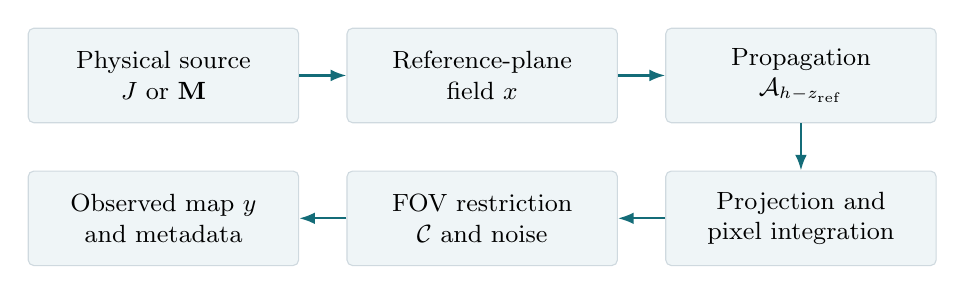
\begin{tikzpicture}[node distance=6mm]
\node[block] (src) {Physical source\\$J$ or $\mathbf M$};
\node[block,right=of src] (ref) {Reference-plane\\field $x$};
\node[block,right=of ref] (prop) {Propagation\\$\A_{h-z_{\rm ref}}$};
\node[block,below=of prop] (sense) {Projection and\\pixel integration};
\node[block,left=of sense] (crop) {FOV restriction\\$\C$ and noise};
\node[block,left=of crop] (obs) {Observed map $y$\\and metadata};
\draw[arrow] (src)--(ref);\draw[arrow] (ref)--(prop);
\draw[arrow] (prop)--(sense);\draw[arrow] (sense)--(crop);\draw[arrow] (crop)--(obs);
\end{tikzpicture}
\caption{The observation model. Generate the physical field on a larger domain before sensing and cropping. The learned inverse estimates the target field and calibration parameters from the observed map.}
\end{figure}

\subsection{Analytical propagation and sensitivity to distance}
In a homogeneous source-free region, $\nabla\times\mathbf H=0$ and $\nabla\cdot\mathbf H=0$. The scalar potential is harmonic. For spatial frequency $\mathbf f=(f_x,f_y)$ in cycles per micrometre,
\begin{equation}
 \widehat x(\mathbf f,z_2)=e^{-2\pi\norm{\mathbf f}(z_2-z_1)}\widehat x(\mathbf f,z_1).
\end{equation}
The three signed components share this decay. In vacuum, $\mathbf B=\mu_0\mathbf H$; store which quantity and units are supplied. In this project the cache is in tesla and loading typically converts to microtesla. $B_{\rm norm}$ is nonlinear and should not be treated as another independent linear measurement channel.

\begin{equation}
 H_\delta(\mathbf f)=e^{-2\pi\norm{\mathbf f}\delta},\qquad
 \partial_h H_\delta=-2\pi\norm{\mathbf f}H_\delta.
\end{equation}
An overestimate $\Delta h$ in a direct inverse multiplies the reconstructed spectral amplitude by $e^{2\pi\norm{\mathbf f}\Delta h}$. At $f=0.5$ cycles/$\mu$m and $\Delta h=0.2\um$, this factor is about $1.87$. This is an analytical illustration, not a measured error bound for a regularized network.

\begin{figure}[htbp]\centering
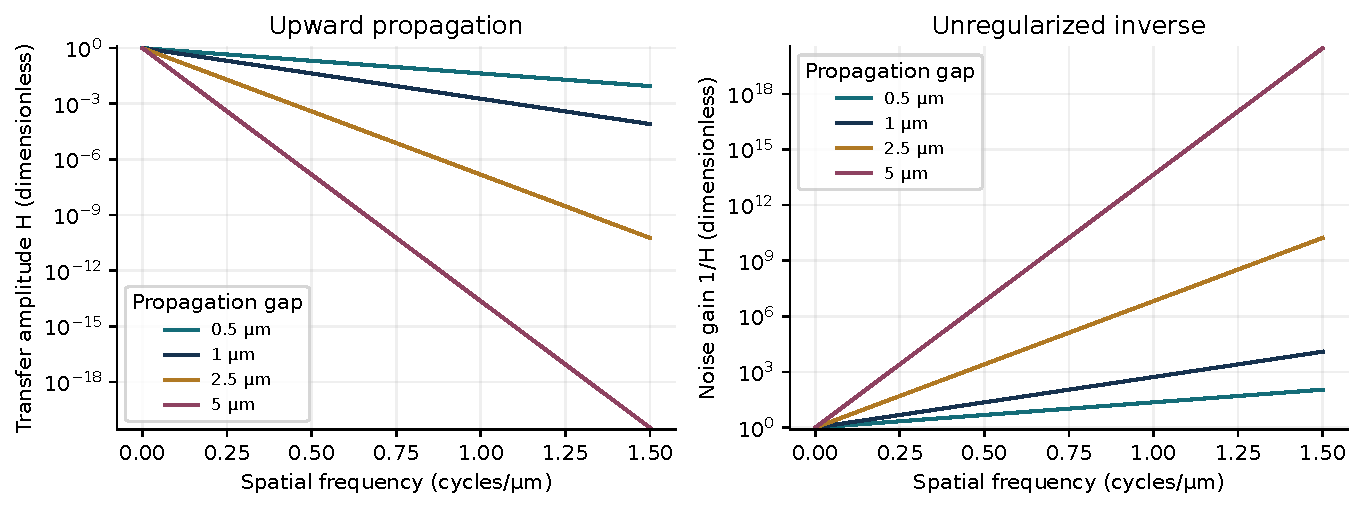
\includegraphics[width=\linewidth]{figures/propagation_and_inverse.pdf}
\caption{Original analytical illustration. Standoff attenuates fine structure and direct inversion amplifies its noise. No experimental reconstruction results are shown.}
\end{figure}
\begin{figure}[htbp]\centering
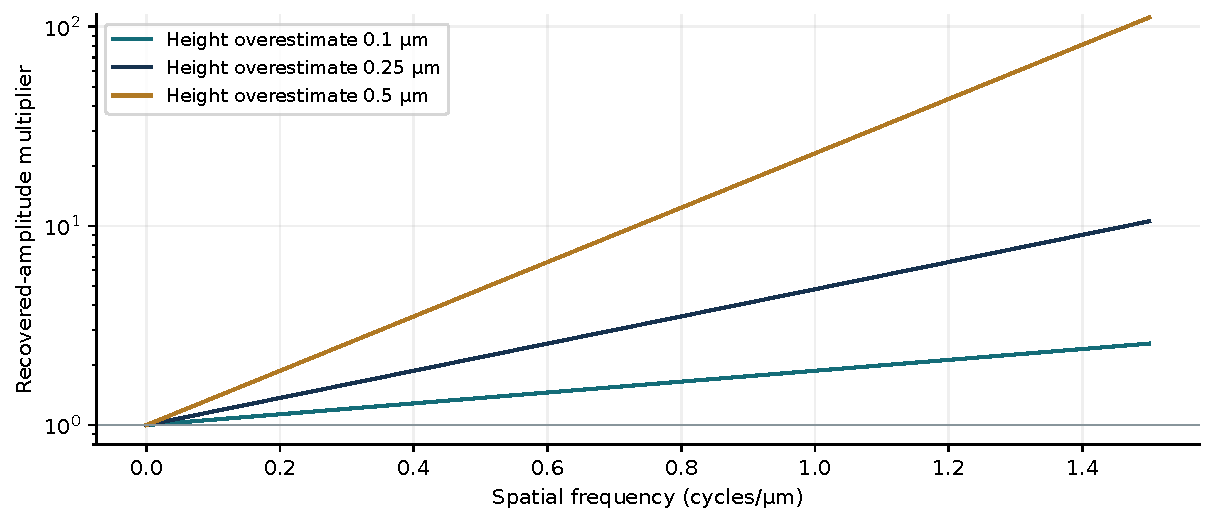
\includegraphics[width=.9\linewidth]{figures/height_sensitivity.pdf}
\caption{Original analytical illustration of distance sensitivity. A fixed height error causes greater spectral distortion at higher frequency. This motivates testing uncertainty-sensitive refinement.}
\end{figure}

\subsection{An exact reason that residual-only height estimation fails}
\begin{figure}[htbp]\centering
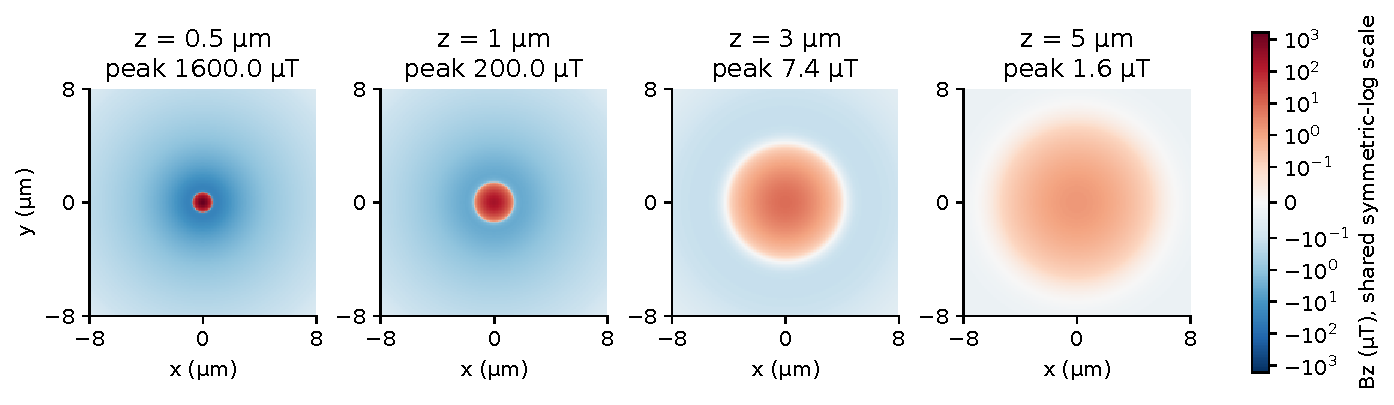
\includegraphics[width=\linewidth]{figures/dipole_height_demo.pdf}
\caption{Original analytical point-dipole example, not a COMSOL or microscope result. A common symmetric-log colour scale exposes both attenuation and broadening; peak values are stated explicitly. This example teaches observation physics, not the proposed coil benchmark.}
\end{figure}
In an ideal infinite-plane, noiseless model, suppose $y=\A_\delta x$. For any $0\leq\delta'\leq\delta$, define $x'=\A_{\delta-\delta'}x$. The semigroup property gives
\begin{equation}
 \A_{\delta'}x'=\A_{\delta'}\A_{\delta-\delta'}x=\A_\delta x=y.
\end{equation}
Thus a smoother reference field at a smaller gap explains the same observation exactly. A flexible unconstrained field can trade source structure against distance. A network trained on one coil size may learn that size as a shortcut and call larger coils ``farther away.''

Restrictions to real source families, geometric knowledge, controlled drive currents, and independent calibration can make height inference informative. A learned estimate is conditional on those assumptions. Physical consistency and extra vector channels improve practical constraints but do not guarantee unique absolute depth for unrestricted planar sources.

\subsection{Profile objectives and nuisance parameters}
A useful diagnostic is
\begin{equation}
 \Phi(h)=\min_x \left\{\tfrac12\norm{W(\mathcal M_hx-y)}^2+\lambda\R(x)\right\},
\end{equation}
where $W$ whitens the assumed noise. Plot $\Phi(h)$, its data term, and ground-truth reconstruction error separately. Profile minima depend on the prior, noise model, support, and solver accuracy; a profile is not automatically a calibrated posterior.

For local source parameters $\vartheta$, define the whitened sensitivities $J_h=\partial_h(W\mathcal M_hx_\vartheta)$ and $J_\vartheta=\partial_\vartheta(W\mathcal M_hx_\vartheta)$. A local nuisance-adjusted information diagnostic is
\begin{equation}
 \mathcal I_{h\mid\vartheta}=J_h^T(I-P_{J_\vartheta})J_h,
\end{equation}
with $P$ the projection onto the nuisance sensitivity span. If distance changes can be reproduced by changing geometry or current, little information remains. This is a local idealized diagnostic; nonlinear multimodality and model error require explicit tests.

\subsection{What additional heights actually provide}
Measurements at several heights above all sources are related by upward continuation in the ideal complete-plane source-free model. They do not independently determine an arbitrary multilayer decomposition. In practice they can improve SNR, registration checks, noise characterization, and finite-window constraints. Known stage increments give relative distances; absolute standoff remains a separate calibration question.

\subsection{A minimal physically constrained source representation}
For planar currents, a stream function $g$ can define $J_x=\partial_y g$ and $J_y=-\partial_x g$, enforcing $\nabla\cdot J=0$ away from contacts. Predicting $g$ and using Biot--Savart provides a source-aware prior, then the field at $z_{\rm ref}$ becomes the main output. Contacts and currents crossing the FOV require appropriate source-domain extensions and boundary treatment. Field-first and source-latent formulations should be compared, not silently conflated.

\caution{Standoff deblurring restores detail conditional on a prior and measurement model. A finer output grid is not evidence of finer physical resolution. Define success through recoverable features, field accuracy, calibration accuracy, and reliability on held-out sources.}

\section{Audit and organize the existing databases}
\label{sec:data}
\subsection{Your resources and the first decisions}
The user confirmed an existing detailed COMSOL database and access to the real measurements from Bathla et al.~\cite{bathla}. The experimental files are on external storage and will be obtained later; their contents have not yet been inspected. The first-paper output is confirmed as near-plane magnetic fields, with currents used as an auxiliary model. Begin the simulation study immediately; make the real-data protocols conditional on the audit rather than postponing the entire project.

\subsection{COMSOL inventory: the first two working days}
Make a read-only manifest before conversion. Give each source layout a stable \texttt{geometry\_id}, and each simulation configuration a \texttt{scene\_id}. Distinguish a genuinely new conductor layout from a different height, current, mesh, or crop of the same layout. Count unique geometries, not exported images.

\begin{longtable}{P{37mm}P{114mm}}
\toprule Required field & Purpose and verification\\\midrule\endhead
Geometry/source identity & CAD/model hash; topology; turns; width; spacing; source layer; contacts. Identify duplicates and translated copies.\\
Coordinates and pitch & Physical $x,y,z$ coordinates; ascending order; exact $\Delta x,\Delta y$; FOV extent. Verify orientation and registration.\\
Height convention & Origin of $z$; conductor top, centre, or substrate reference; known source thickness; absolute height versus gap.\\
Drive & Applied current/voltage; measured or prescribed value; sign; contact boundary conditions.\\
Physics and quantity & $\mathbf B$ versus $\mathbf H$; units; material permeability; current density availability; source-free region validity.\\
Numerics & COMSOL version, mesh size, solver tolerance, interpolation/export procedure, simulation boundaries.\\
Files and provenance & Paths, SHA-256, grid shape, data type, component labels, missing values, source-generation seed.\\
Target availability & Field at $z_{\rm ref}$; existence of complete same-geometry height sweeps; whether a trusted target needs new simulation.\\\bottomrule
\end{longtable}

Create a report showing height counts per geometry, pitch/FOV distributions, missing components, field ranges, and coordinate agreement. Plot a few profiles at every height. Repeated field interpolation artifacts are model discrepancy, not automatically independent measurement noise.

\subsection{Reuse complete height sweeps without learning test-pair kernels}
Where a geometry has fields at $z_{\rm ref}$ and several higher planes, use the lower field as target and each higher plane as an observation. The analytical operator is evaluated from physical spacing and height. A held-out sharp field must not be used to fit that observation's empirical kernel.

Compare direct COMSOL high-plane fields with analytical propagation of the low-plane field. This residual includes export interpolation, discretization, finite-window error, registration, and any modelling mismatch. Investigate its structure before ascribing it to mesh noise. A bounded empirical correction may be a later experiment, but its parameters must be fitted on training/calibration data only, and tested on unused geometries or acquisition sessions.

\subsection{Dataset tiers}
\begin{tabularx}{\linewidth}{P{27mm}YY}
\toprule Tier & Data & Scientific role\\\midrule
T0: mechanics & Small analytical cases, Fourier modes, closed loops & Operator, adjoint, gradients, and ambiguity checks\\
T1: pilot & Stratified subset of the existing COMSOL database & Baseline comparison and failure discovery\\
T2: challenge & Disjoint COMSOL layouts/families and selected numerical settings & Generalization; simulator/model mismatch\\
T3: real archive & Audited Bathla maps, labels, and repetitions & Real noise, dictionary comparison, source activations\\
T4: new acquisition & Calibrated height sweeps and independent layouts & Direct validation of target-plane reconstruction and distance\\\bottomrule
\end{tabularx}
Use new analytical scenes to answer controlled questions, not as a replacement for the existing database. Add new COMSOL simulations only to fill an identified gap: geometry families, near-plane references, mesh-convergence checks, or height ranges.

\subsection{Splitting protocol and leakage controls}
First assign source identities to train, validation, calibration, and test groups; only then derive heights, current rescalings, crops, and noise variants. The calibration group is needed only if uncertainty calibration is included and must be distinct from the model-selection validation set. All descendants of a geometry remain in the same group. Near-duplicates and variants from the same template generator may require a higher-level family grouping.

Maintain two different evaluations: \textbf{new-instance interpolation} within a geometry family, and \textbf{unseen-family transfer}. A random split of configurations is not evidence of unseen geometry. Separate height interpolation from extrapolation. Record exact withheld ranges and test them once after selecting the model.

\begin{figure}[htbp]\centering
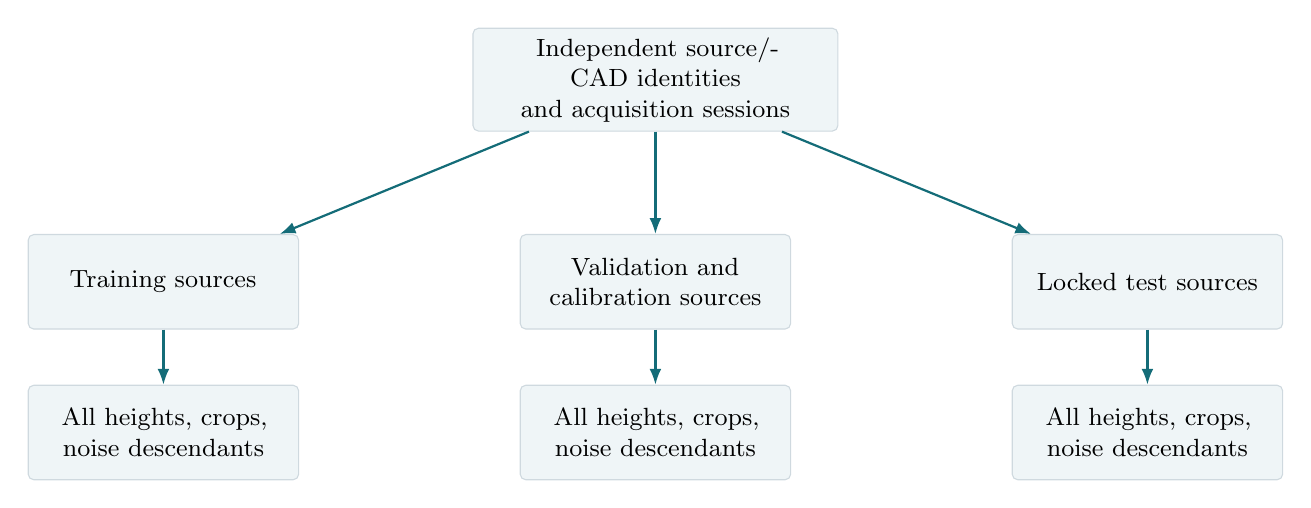
\begin{tikzpicture}[node distance=7mm]
\node[wideblock] (ids) {Independent source/CAD identities\\and acquisition sessions};
\node[block,below left=13mm and 22mm of ids] (train) {Training sources};
\node[block,below=13mm of ids] (val) {Validation and\\calibration sources};
\node[block,below right=13mm and 22mm of ids] (test) {Locked test sources};
\node[block,below=of train] (td) {All heights, crops,\\noise descendants};
\node[block,below=of val] (vd) {All heights, crops,\\noise descendants};
\node[block,below=of test] (ed) {All heights, crops,\\noise descendants};
\draw[arrow] (ids)--(train);\draw[arrow] (ids)--(val);\draw[arrow] (ids)--(test);
\draw[arrow] (train)--(td);\draw[arrow] (val)--(vd);\draw[arrow] (test)--(ed);
\end{tikzpicture}
\caption{Split physical identities before creating training examples. Correlated crops and height variants cannot be moved across source-level partitions.}
\end{figure}

For a pilot, choose approximately 100 independent layouts \emph{if available}, with a 60/20/20 source-level train/validation/test split. This is a starting engineering configuration, not a sample-size justification. If calibration is needed, reserve additional sources or repartition without examining the locked test outcomes. Expand according to learning curves and precision of source-level confidence intervals.

\subsection{Sampling, cropping, and normalization}
Propagate on a larger domain and then apply pixel integration and FOV restriction. For coarser pitch, antialias and integrate the field; do not simply resize an image and declare a new physical spacing. Upsampling labels does not create new measured information. If the target uses a different grid, make that output grid explicit and interpolate only through a documented observation model.

Use a fixed scale estimated from training data or an observation-only scale $q(y)$, and retain $q$ as physical metadata when amplitude carries information. Reconstruct in physical units for metrics. If minimizing the existing half-squared loss plus an L1 penalty under $x=q u$, the normalized coefficient is $\lambda/q$. Do not normalize using held-out sharp targets. At zero or near-zero signal, use a predetermined scale floor and flag height as uninformative.

Rotating a field image requires rotating its vector components as well as its spatial coordinates. Under a planar rotation $R$, rotate $(B_x,B_y)$ consistently and transform the NV projection direction for scalar observations. Scaling geometry changes physics and cannot be implemented by spatial resizing alone. Reverse all signed components for current reversal under the linear magnetostatic model.

\section{How to use Anuj Bathla's experimental dataset}
\label{sec:bathla}
\subsection{What is established and what is still unknown}
The published study describes measured individual-coil basis fields and mixed activations on a multilayer micro-coil platform, plus time-dependent measurements. Its reconstruction uses sparse coefficients in a measured dictionary. Your group's original files may contain more information than the paper, but this guide cannot assume that fixed-reference sharp fields, absolute calibrated standoffs, or all vector components are already present. Obtain those facts from acquisition logs.

\subsection{Data-receipt checklist}
\begin{enumerate}
\item Copy data into a read-only archive; retain original folder structure, checksums, and the acquisition notebook. Work from versioned derived copies.
\item Identify field maps, raw ODMR/lock-in sequences, current-on/off references, individual-coil maps, mixed activations, timestamps, and event waveforms.
\item Obtain the coil-to-layer lookup, microscope magnification, pixel pitch, NV axis, coordinate conventions, drive values, and registration transforms.
\item Label every distance as independently measured, nominal, model-fitted, relative stage displacement, or unknown. Store uncertainty and calibration method.
\item Ask whether basis maps and mixtures were measured in the same session and at the same drive. Check drift, gain, and background differences.
\item Verify data-release permission and what can be made public. This affects the reproducibility package; it does not alter the scientific split.
\end{enumerate}

\subsection{Six concrete uses, in increasing order of difficulty}
\textbf{U1: benchmark the published task.} Reproduce field fitting and activation recovery with the measured dictionary before adding a neural network. The unknown is a coefficient vector, not field pixels. For dictionary $D=[d_1,\ldots,d_K]$ and observation $y$, solve
\begin{equation}
 \hat c=\arg\min_c \tfrac12\norm{W(Dc-y)}^2+\lambda\norm{c}_1.
\end{equation}
Use NNLS only if nonnegative currents are physically justified. Compare coefficient error, activation precision/recall, and field residuals. This is a calibration and reproducibility exercise, not a new research claim.

\textbf{U2: learn experimental noise.} Repetitions and current-off acquisitions can estimate spatial variance, correlations, drift, and fitting uncertainty. Subtracting a spatially varying physical field is not equivalent to measuring noise. Split sessions so repeated backgrounds do not leak. Where raw ODMR fits provide covariance, propagate it or use it to weight the observation loss.

\textbf{U3: calibrate simulator-to-measurement discrepancy.} Match known CAD and drive settings to measured individual-coil fields. Fit limited nuisance parameters such as global registration, axis angle, gain, and effective distance on a calibration subset. Do not allow a free learned kernel to absorb every error. Test fitted corrections on unused coils or sessions.

\textbf{U4: experimentally adapt a pretrained field prior.} Start from COMSOL supervision. Use repeated real observations, known source activations, and correctly modelled measurement consistency to adapt on an explicit adaptation set. Validate on separate acquisitions. A dictionary-generated $D c$ is a \emph{model-based surrogate at the sensor plane}, not an independent near-plane truth. Shared noisy basis maps can correlate surrogate target and input noise.

\textbf{U5: construct a real dictionary LISTA baseline.} Train an unrolled sparse-code network for $c$ on activation labels and compare with LASSO at matched inference latency. This tests learned acceleration and provides a source-aware auxiliary branch. It does not directly establish standoff super-resolution. Hold out activation patterns for known-dictionary performance; hold out source identities or a new array for geometry transfer.

\textbf{U6: validate near-plane reconstruction.} If the archive contains registered measurements at several calibrated positions, form higher-to-lower-plane test pairs with the same optics. Otherwise acquire new height sweeps. Do not invent sharp references by applying your own inverse to the archive and then evaluate against them.

\begin{figure}[htbp]\centering
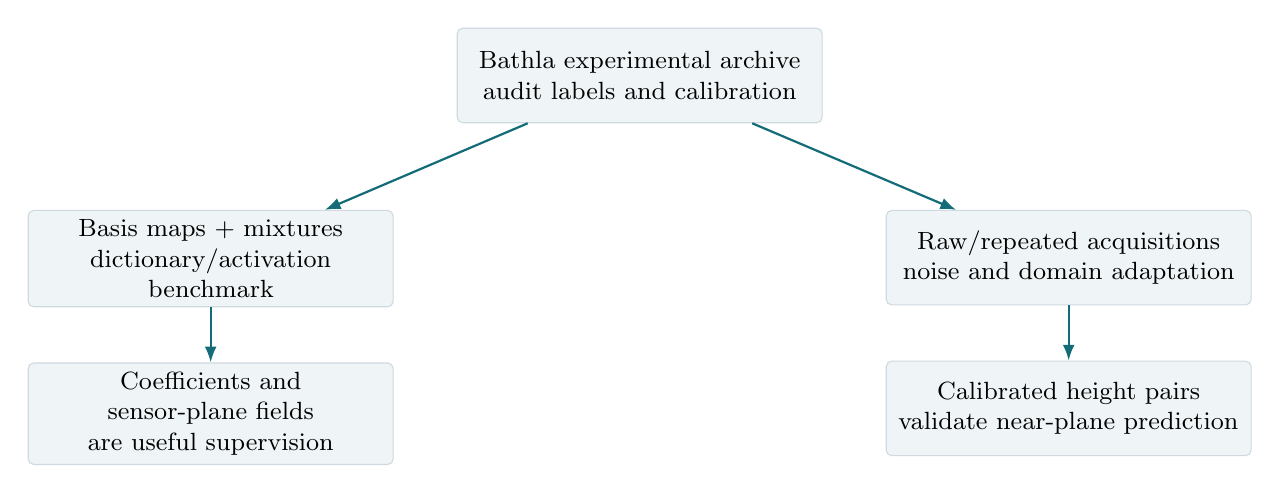
\begin{tikzpicture}[node distance=7mm]
\node[wideblock] (archive) {Bathla experimental archive\\audit labels and calibration};
\node[wideblock,below left=11mm and 8mm of archive] (known) {Basis maps + mixtures\\dictionary/activation benchmark};
\node[wideblock,below right=11mm and 8mm of archive] (repeat) {Raw/repeated acquisitions\\noise and domain adaptation};
\node[wideblock,below=of known] (labels) {Coefficients and sensor-plane fields\\are useful supervision};
\node[wideblock,below=of repeat] (sweep) {Calibrated height pairs\\validate near-plane prediction};
\draw[arrow] (archive)--(known);\draw[arrow] (archive)--(repeat);
\draw[arrow] (known)--(labels);\draw[arrow] (repeat)--(sweep);
\end{tikzpicture}
\caption{Different experimental data support different claims. Activate a branch only after the necessary metadata and measurements are verified.}
\end{figure}

\subsection{Splits that are honest for a single fabricated array}
Holding out activation combinations tests combinatorial generalization for \emph{known source templates}. All combinations on one array are not independent new geometries. A shared dictionary may be legitimate calibration information in that task, but it must be declared and kept separate from unseen-geometry claims. Use held-out acquisition sessions to test drift. For dynamics, split contiguous events/runs and leave guard intervals; neighbouring frames are strongly correlated.

If a known-coil dictionary is available at test time, report that regime separately from ``no per-coil calibration.'' Holding out a coil while secretly supplying its measured basis is not unknown-source generalization. For unseen coils, use CAD-based physical templates or new independent arrays and disclose the information provided.

\caution{A known activation vector can label which source was driven; it does not necessarily give an exact current amplitude or a unique multilayer current map. Model-assisted labels, nominal heights, and independently measured targets should appear as separate evidence tiers.}
\deliver{Produce two manifests, a source/session split file, a dictionary reproduction report, and a list of missing metadata or acquisitions needed for the primary near-plane claim.}

\section{The experiment ladder: investigate before inventing}
\label{sec:experiments}
Each experiment should have a short configuration file, immutable split identifier, source revision, arrays, metrics, and a visual report. Work through E00--E05 first. The remaining experiments are selected by the observed failure, rather than executed as an indiscriminate architecture sweep.

\subsection{E00: operator correctness and model discrepancy}
\textbf{Question.} Does the observation operator represent the data well enough that a new network is scientifically interpretable?

\textbf{Procedure.} Check Fourier-mode attenuation, identity at zero gap, nonnegative upward gaps, padding/cropping, pixel integration, component projection, and transpose ordering. Verify $\langle\mathcal M_hx,r\rangle=\langle x,\mathcal M_h^*r\rangle$ on asymmetric grids and masks. Compare the autograd derivative in $h$ with centred finite differences on a small problem. Compare independent COMSOL high-plane fields with propagated reference fields, using interior and full-FOV metrics.

\textbf{Controls.} Increase physical-domain size/padding; refine one representative COMSOL mesh; compare registered coordinates. Test double precision on a small case before using GPU float32. If error changes with window size, do not call it solely simulation noise.

\textbf{Output.} Adjoint/gradient errors, component residual maps, residual spectra, interior-versus-boundary error, and a model-discrepancy summary. This step is a necessary numerical verification, not a novel result by itself.

\subsection{E01: known-height reconstruction}
\textbf{Question.} What detail is recoverable when calibration is available?

Run analytic filtered inversion, classical regularized reconstruction, the repository's LISTA with physics corrections, and a small supervised residual CNN or U-Net on the same source split. Use the true height only in the explicitly labelled known-height controls. Tune cutoffs and penalties on validation sources. Evaluate every component, a predefined source ROI, profiles, and latency.

Compare field-pixel L1, quadratic smoothness, wavelet sparsity, and vector TV as distinct priors. For vector TV one possible definition is
\begin{equation}
 \R_{\rm VTV}(x)=\sum_p\sqrt{\sum_c[(D_xx_c)_p^2+(D_yx_c)_p^2]+\varepsilon_{\rm TV}^2}.
\end{equation}
Choose finite-difference spacing in physical units. An arbitrary CNN denoiser is not automatically a proximal operator, and its iterations do not inherit FISTA's convex convergence guarantee.

\gate{If known-height methods cannot recover the target on the pilot, investigate noise, sampling, source prior, or model mismatch before introducing height estimation. A known-height control is an information reference, not a universal accuracy upper bound.}

\subsection{E02: intentionally wrong height}
\textbf{Question.} How much does calibration error affect reconstruction, and can residuals diagnose it?

Select low, medium, and high heights from the actual database and multiple independent layouts. Sweep assumed height around each true value, subject to $h>z_{\rm ref}$. For an observation at $3\um$, an illustrative sweep is $2$ to $4\um$ with finer samples near $3\um$. Reconstruct to the same declared solver tolerance at each candidate. Reuse warm starts only if their effect and timing are recorded.

Plot reconstruction error, whitened observation mismatch, regularization cost, and feature/profile error against assumed height. Repeat at zero noise and two specified physical noise levels. Show cases where a good residual accompanies a poor reconstruction.

\textbf{Interpretation.} A broad residual valley is consistent with ambiguity; a narrow prior-dependent objective minimum does not establish true height. A monotone preference for the lowest permitted height may reflect the semigroup degeneracy. Use this experiment to set application-relevant error tolerances rather than inventing a success threshold after seeing test data.

\subsection{E03: source--height ambiguity and shortcut detection}
\textbf{Question.} Which changes in source parameters can imitate a height change?

Vary source size, track width, turns, spacing, location, and current independently of height. Find nearest observation pairs from different layouts/heights using a noise-weighted distance. For Gaussian noise a likelihood comparison uses the whitened separation $\norm{\Sigma^{-1/2}(y_1-y_2)}$; interpret it under the actual covariance and sampling, not raw pixel count. Verify lookalike cases visually and using profiles.

Train a minimal height predictor. Evaluate it on held-out size ranges, current amplitudes, and shape families. Compare physical units, observation-only normalization with retained amplitude, and normalization that discards amplitude. Do not discard amplitude and then conclude that it is irrelevant.

\textbf{Output.} An ambiguity gallery; height error by geometry/current subgroup; predictive spread on lookalikes; and a labelled subset of informative versus weakly informative cases. These cases should remain fixed for comparing later models.

\subsection{E04: the two-stage baseline}
\textbf{Question.} Is a simple height estimator followed by reconstruction sufficient?

Train a CNN encoder with global pooling and an MLP receiving physical metadata. Predict $h$ within the allowed training interval. Feed its estimate to a conditioned reconstructor trained with known heights. Evaluate a second variant in which the reconstructor is trained using noisy height estimates matching the predictor's validation errors; otherwise a brittle two-stage baseline can make joint inference look unfairly strong.

Compare height MAE, field error, failure rate, and latency with the known-height counterparts. Repeat with at least several model seeds once the pilot is stable. Use the same prior capacity and training budget wherever feasible.

\subsection{E05: joint field--height refinement}
\textbf{Question.} Does feedback between calibration and reconstruction add value?

Start from the two-stage initialization, then perform a small trained number of physics-and-prior refinement stages. Supervise both height and reference field on simulation data; include observation consistency. Compare (a) frozen height, (b) gradient height updates, and (c) learned residual-based height updates. Control total parameter count and inference compute, not only stage count.

\textbf{Required ablations.} Same reconstruction prior; identical metadata; same dataset; matched height initialization; no-refinement model trained end to end; and a larger two-stage model under a similar compute budget. Log intermediate heights and errors to detect unstable oscillations or drift toward the bound.

\gate{Advance to a novel mechanism only if there is a reproducible residual failure: ambiguity, noise amplification, scale mismatch, boundary inconsistency, or simulation-to-real mismatch. If the strong two-stage model solves the task, develop a different scientific claim instead of obscuring it with added modules.}

\subsection{E06: multiple hypotheses and calibrated rejection}
Compare one height estimate with a coarse candidate bank and a shared conditional reconstructor. Preserve associated pairs $(x_j,h_j)$ instead of mixing unrelated image and height averages. Evaluate true-height set coverage, interval/set width, conditional coverage by geometry/noise, and the error on cases retained at increasing confidence thresholds. Compare with a small ensemble and simple grid-search profiling.

For discrete candidates, report the approximation error due to binning and include heights between training bins. Use a separate calibration set for temperature scaling or conformal adjustments. The ability to return broad sets is useful only when informative cases remain narrow and difficult cases are reliably flagged.

\subsection{E07: FOV, pitch, and outside-window contributions}
Use a full physical scene as the common parent. Create (i) different crops at fixed pitch, (ii) different pitches at fixed physical FOV, and (iii) different FOVs at fixed array dimensions. These are three different shifts. Integrate and antialias before subsampling. Compare on registered common physical regions with documented target-grid conversion.

Test sources touching the edge and sources just outside the window. Compare zero exterior, increased latent-domain support, and an explicit nuisance exterior model. Measure interior error, edge-band error, overlap disagreement, height bias, and predictive uncertainty. Cropping a propagated image is not equivalent to propagating a crop.

\subsection{E08: noise and acquisition robustness}
Start with known white Gaussian noise as a controlled experiment, then add correlated noise, spatially varying variance, offsets, and drift estimated from real repetitions. Keep physical noise level distinct from SNR; increasing height reduces signal even if instrument noise remains fixed. Test both fixed-noise and fixed-SNR protocols, labelled separately.

For repeated measurements, independent noise can support noise-to-noise denoising or adaptation, but does not by itself reveal frequencies removed by standoff. Check shared calibration noise, fitting-induced spatial correlation, and drift before assuming conditional independence. QDsiM~\cite{qdsim} provides a noise-aware measurement simulation reference; adopting a simulator alone is not a methodological novelty.

\subsection{E09: COMSOL-to-experiment transfer}
Match scalar NV projection versus vector input, units, sensor averaging, and acquisition backgrounds. Train on COMSOL, evaluate without adaptation, then compare calibration-only adaptation and learned-prior adaptation on disjoint real sessions. Include a small real-only control if independently labelled height pairs are available. Separate gains from registration/calibration improvements from gains due to the new architecture.

\subsection{E10: physical resolution and prior dependence}
Define a controlled feature family: for example two nearby track contributions, a narrow gap, or a small perturbation on a known source. Sweep separation and SNR at several heights. Define a detection or profile criterion before locking the test set; report false positives and confidence, not just visual sharpness. Compare ordinary interpolation to rule out claims based solely on increased output pixels.

Perturb the learned prior with plausible out-of-distribution layouts. If features appear in the reconstruction without support in the measurement, test whether the uncertainty mechanism flags them. A successful resolution claim must state the source family and measurement conditions under which it holds.

\subsection{E11: optional sensor tilt and effective averaging}
If constant-height inference fails systematically across the FOV, use a low-dimensional tilted plane $h(x,y)=h_0+a x+b y$. Evaluate the physical field on the nonplanar measurement coordinates and rotate the projection axis consistently when required. A spatial height map is not implemented by naively applying a different local convolution at each pixel. Compare with a scalar effective-height model on controlled simulated tilt and independently characterized acquisitions.

\subsection{E12: optional multilayer source separation}
Only after single-layer validation, model $y=\sum_\ell\mathcal M_{h_\ell}x_\ell+\eta$, preferably with structural source priors or known template families. Use the Bathla dictionary as the known-source baseline. Add continuous depth/position corrections and test dictionary mismatch. Report cross-talk, activity errors, layer-parameter uncertainty, and information supplied at inference. Arbitrary layer images at arbitrary depths are not uniquely identifiable from one sum.

\begin{figure}[htbp]\centering
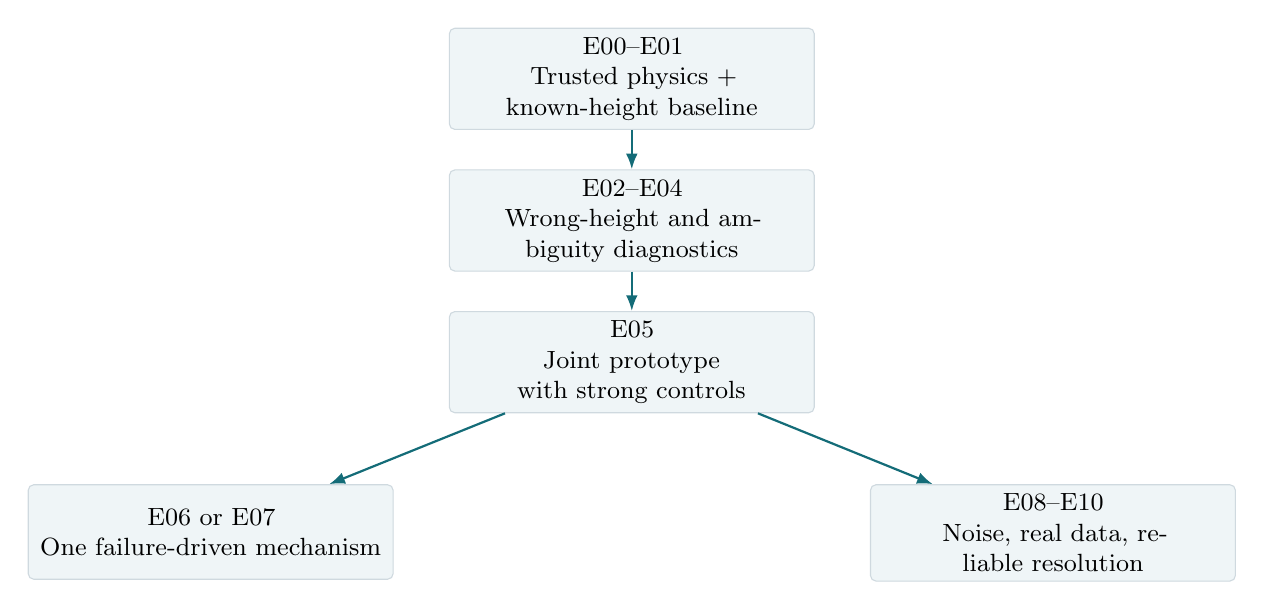
\begin{tikzpicture}[node distance=5mm]
\node[wideblock] (op) {E00--E01\\Trusted physics + known-height baseline};
\node[wideblock,below=of op] (fail) {E02--E04\\Wrong-height and ambiguity diagnostics};
\node[wideblock,below=of fail] (joint) {E05\\Joint prototype with strong controls};
\node[wideblock,below left=9mm and 7mm of joint] (novel) {E06 or E07\\One failure-driven mechanism};
\node[wideblock,below right=9mm and 7mm of joint] (real) {E08--E10\\Noise, real data, reliable resolution};
\draw[arrow] (op)--(fail);\draw[arrow] (fail)--(joint);\draw[arrow] (joint)--(novel);\draw[arrow] (joint)--(real);
\end{tikzpicture}
\caption{A research ladder with decision gates. E11--E12 are optional extensions, not prerequisites for completing the first paper.}
\end{figure}

\deliver{Maintain one experiment ledger with IDs E00--E12, question, control, split, configuration hash, primary metrics, figure, conclusion, and next decision. A failed hypothesis is retained with its evidence.}

\section{What architectures to learn, build, and compare}
\label{sec:architectures}
\subsection{A learning order tied to implementation milestones}
\begin{longtable}{P{26mm}P{57mm}P{68mm}}
\toprule Learn in order & Concept and reference & Implement and explain before moving on\\\midrule\endhead
1. Proximal inference & ISTA/FISTA and LISTA~\cite{lista}; ALISTA~\cite{alista} & Derive the gradient, adjoint, shrinkage, and step bound; distinguish optimization error from field error.\\
2. Residual CNN & Signed regression and residual prediction & A small known-height field reconstructor; linear output, correct units, sensible initialization.\\
3. U-Net & Multiscale encoder/decoder with skip paths~\cite{unet} & Compare local CNN and multiscale context; separate architecture choice from supervised training target.\\
4. Conditioning & Feature modulation, e.g. FiLM~\cite{film} & Condition on physical height/pitch/noise, and prove with an ablation that metadata improves transfer.\\
5. Learned data consistency & MoDL~\cite{modl} and VarNet~\cite{varnet} as transferable patterns & Combine a learned prior with the exact measurement operator, including crop and projection.\\
6. Blind inference & Joint image/operator estimation~\cite{blinddps} & A bounded height update; diagnose prior-dependent calibration and degenerate solutions.\\
7. Uncertainty & Calibration~\cite{guo}; conformal prediction~\cite{conformal} & Coverage and sharpness on a held-out calibration set; detect distribution-shift failures.\\
8. Optional priors & DIP~\cite{dip}, plug-and-play~\cite{pnp}, FNO~\cite{fno} & Try only when the current failure suggests scan-specific fitting, stronger priors, or operator transfer.\\\bottomrule
\end{longtable}
For each reading, write half a page: variables estimated, prior, measurement operator, information supplied at test time, data split, and a failure relevant to QDM. Architecture labels do not replace this analysis.

\subsection{A0: reproduce the existing physics-correction LISTA}
The repository currently uses
\begin{equation}
 x_{k+1}=\operatorname{soft}_{\theta}\left[x_k-\alpha A^*(Ax_k-y)+C_b y+C_x x_k\right].
\end{equation}
Its two bias-free $9\times9$ single-channel corrections and scalar threshold are tied across layers. It has 163 trainable parameters, and zero corrections reproduce ISTA at initialization. $H$ is fixed in the current checkpoint/operator. Supervision targets sharp fields rather than sparse-optimization solutions; the distinction from original LISTA~\cite{lista} matters.

\textbf{Useful first ablations.} Train versus zero correction; tied versus untied thresholds; input correction versus state correction; scalar versus per-component threshold; same physical prior at several trained depths; blurred versus zero initialization. Compare accuracy--latency curves. A trained layer has extra convolutions, so it is not equal in cost to an ISTA iteration. Preserve the trained-depth restriction and do not infer convergence of learned updates.

\textbf{A controlled LISTA study you can run before the joint model.} Use trained depths $K\in\{4,8,16\}$ as an illustrative pilot grid, and compare (i) fixed true-height ISTA/FISTA, (ii) zero-correction LISTA, (iii) trained tied corrections, (iv) learn only steps/thresholds, and (v) untied corrections. Log field error after each trained stage, physical residual, learned parameter changes, inference memory, and latency. Select the depth on validation sources. The fixed-depth classical controls diagnose acceleration; epsilon-stopped classical controls diagnose optimization. They answer different questions and should both be reported.

A learned-FISTA control can introduce bounded trained momentum into the same physics update. Treat it as a fixed-depth network; classical FISTA guarantees do not automatically apply to learned momentum or learned priors. If a compact step/threshold model matches a larger correction network, that is evidence to simplify the prior, not a reason to hide the smaller control.

\subsection{A0b: coefficient LISTA for the Bathla dictionary}
This is a distinct task with a genuinely sparse representation:
\begin{equation}
 c_{k+1}=\operatorname{soft}_{\tau_k}\left(c_k+\alpha_k D^TW^TW(y-Dc_k)\right).
\end{equation}
Learn bounded steps/thresholds first, then consider learned corrections. Inputs are measured projected maps; outputs are coil coefficients. Compare with LASSO, ridge, and applicable sign-constrained fits using activation labels. Derive near-plane fields only through independently validated physical source templates. A measured sensor-plane basis cannot itself supply a sharp reference-plane basis.

\subsection{A1: supervised residual CNN and U-Net controls}
Use a small residual CNN with approximately 4--6 convolutional blocks and 32--64 feature channels as an initial engineering configuration. A U-Net control can use 3--4 scales and comparable capacity. Predict $\hat x=x_0+R_\theta(y,m)$ with a linear final layer, where $m$ is metadata and $x_0$ is a declared physical or observation-derived initialization.

Train from scratch on magnetic data. Natural-image priors and pretrained RGB weights can impose unsuitable textures. Do not use sigmoid output for signed microtesla fields. Avoid hidden resizing, instance normalization that discards meaningful amplitude, and random-crop training that silently changes the forward boundary conditions. Compare fixed amplitude metadata versus observation normalization with scale retained.

Learn that a convolutional architecture is not automatically FOV/pitch invariant: a $9\times9$ kernel spans different physical distances as pitch changes. Global pooling for height estimation can also hide how much of a source is visible. Test these issues rather than claiming invariance from variable tensor dimensions.

\subsection{A2: known-height conditioned physics network}
Let $r_k=\mathcal M_hx_k-y$, and define
\begin{align}
 u_k &= x_k-\alpha_k\mathcal M_h^*W^TW r_k,\\
 x_{k+1}&=u_k+R_\theta(u_k,\mathcal M_h^*W^TW r_k;m).
\end{align}
Condition the learned correction using a small metadata MLP. One FiLM-style implementation modulates feature channel $j$ by $\gamma_j(m)z_j+\beta_j(m)$. Proposed metadata include physical $\Delta x,\Delta y$, gap, noise estimates, amplitude scale, projection/channel availability, and observation mask. Standardize metadata using training statistics.

Start with 6--8 stages, tied correction weights, and a conservative bounded step. These are pilot choices, not optimal hyperparameters. In a whitened problem the norm bound includes $W$, sampling, and projection; do not reuse the bound for an unweighted convolution. Removing conditioning, physics gradients, or stage tying gives informative controls.

An alternative MoDL-style data-consistency block solves
\begin{equation}
 (\mathcal M_h^*W^TW\mathcal M_h+\rho I)x_{k+1}
 =\mathcal M_h^*W^TW y+\rho D_\theta(x_k;m)
\end{equation}
approximately using conjugate gradients. For padded/cropped operators, apply the true composition rather than replacing it by multiplication with $|H|^2$. Report CG accuracy and its contribution to runtime; keep $\rho>0$.

\subsection{A3: a strong two-stage calibration baseline}
A height encoder produces $h_0=h_{\min}+(h_{\max}-h_{\min})\operatorname{sigmoid}(s_\phi(y,m))$. Define this admissible physical interval independently of the training range; it can be broader than the training heights. Extrapolation tests must remain within the declared interval, and observations outside it are flagged as unsupported. Feed the estimate to A2. Train the predictor on true simulation labels and the reconstructor first on correct heights, then on realistic predictor errors. Jointly training the two blocks without iterative height feedback is a stronger control than freezing a poorly trained predictor.

For a scalar NV input, use the proper projection in $\mathcal M_h$ and a channel-availability mask. Vector outputs inferred from a scalar image require corresponding physical assumptions and can only be validated in channels with trusted reference data. Do not use current amplitude, source CAD, or true height in the network unless the inference regime declares them available.

\subsection{A4: joint refinement prototype}
Given $(x_k,h_k)$, perform the A2 field update and refine height. A physics-only candidate is
\begin{align}
 g_{h,k}&=\left\langle W r_k,W\,\partial_h\mathcal M_{h_k}x_k\right\rangle,\\
 h_{k+1}&=\Pi_{[h_{\min},h_{\max}]}(h_k-\beta_k g_{h,k}).
\end{align}
An alternative learns a bounded correction from $r_k$, $x_k$, metadata, and residual spectral summaries. Use explicit supervision for $h$ and $x$ during simulation training. The residual gradient is a useful feature, but does not resolve non-identifiability by itself. A learned source prior or source-latent representation supplies additional restrictions.

\begin{figure}[htbp]\centering
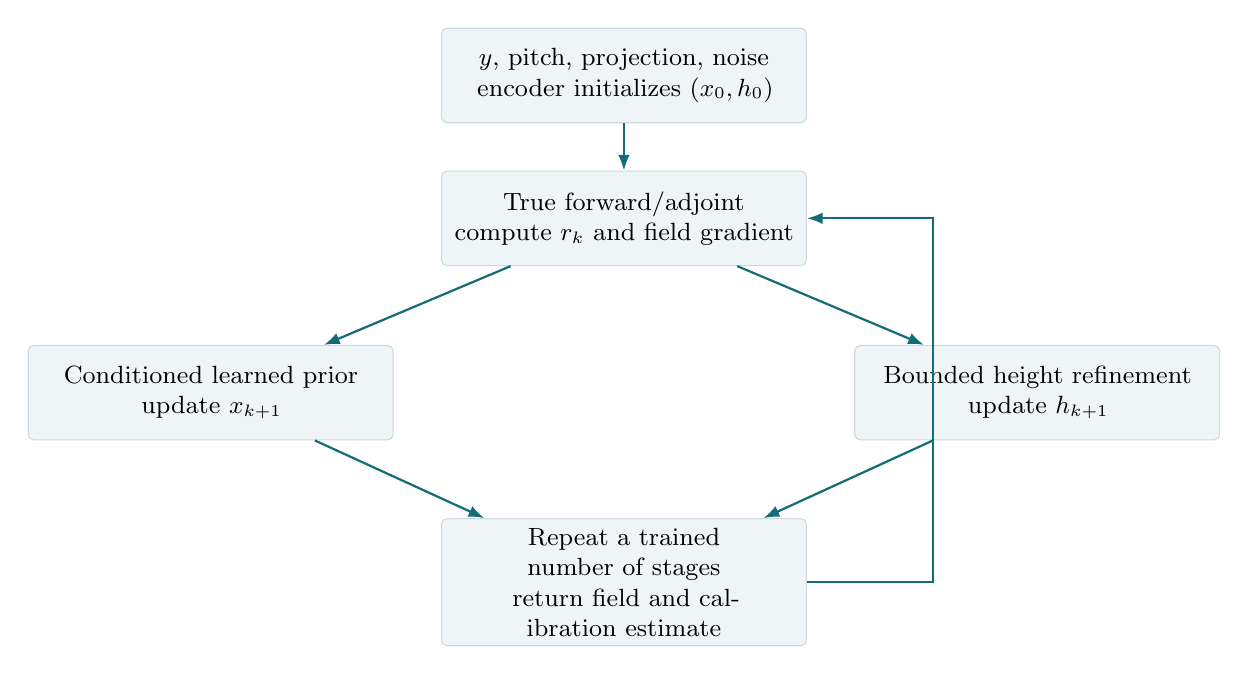
\begin{tikzpicture}[node distance=6mm]
\node[wideblock] (init) {$y$, pitch, projection, noise\\encoder initializes $(x_0,h_0)$};
\node[wideblock,below=of init] (physics) {True forward/adjoint\\compute $r_k$ and field gradient};
\node[wideblock,below left=10mm and 6mm of physics] (prior) {Conditioned learned prior\\update $x_{k+1}$};
\node[wideblock,below right=10mm and 6mm of physics] (height) {Bounded height refinement\\update $h_{k+1}$};
\node[wideblock,below=32mm of physics] (out) {Repeat a trained number of stages\\return field and calibration estimate};
\draw[arrow] (init)--(physics);\draw[arrow] (physics)--(prior);\draw[arrow] (physics)--(height);
\draw[arrow] (prior)--(out);\draw[arrow] (height)--(out);
\draw[arrow] (out.east) -- ++(16mm,0) |- (physics.east);
\end{tikzpicture}
\caption{Proposed joint prototype. The exact operator handles known physics; the learned block encodes a data-dependent prior. Both height and reconstruction are trained and evaluated explicitly.}
\end{figure}

Do not change the analytical operator with unconstrained learned filters and simultaneously call the resulting scalar a physical distance. If adding $H_{\rm eff}=H_h+\Delta H_\psi$, bound and calibrate $\Delta H_\psi$, check Hermitian symmetry/reality, and test whether the correction absorbs height. Compare the pure analytical model, a calibration-only correction, and a trained correction on source/session holdouts.

\subsection{A5: a candidate bank for ambiguous height}
Choose an initial set of plausible heights $\{h_j\}_{j=1}^J$ and share the A2 reconstructor across candidates. Predict or optimize a field $x_j$ for each, then score the pairs using measurement likelihood and a learned source prior. A conceptual Bayesian score is
\begin{equation}
 \log p(h_j,x_j\mid y)\propto
 -\tfrac12\norm{W(\mathcal M_{h_j}x_j-y)}^2+\log p_\theta(x_j)+\log p(h_j).
\end{equation}
This equation is not a justification for calling arbitrary network logits a posterior. If $p_\theta$ is unavailable as a normalized density, label scores as predictive weights and calibrate empirically. Height classification on true labels is a simple initial implementation. Then test continuous refinement, bin-width effects, and branch collapse.

\begin{figure}[htbp]\centering
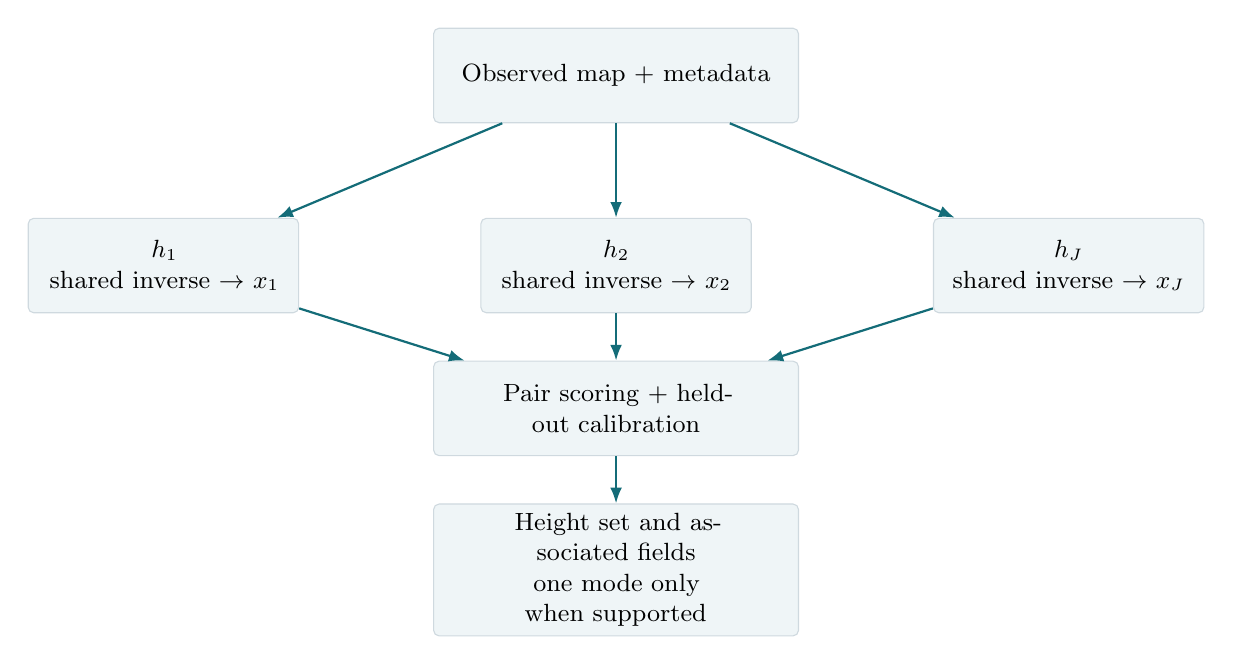
\begin{tikzpicture}[node distance=6mm]
\node[wideblock] (in) {Observed map + metadata};
\node[block,below left=12mm and 17mm of in] (b1) {$h_1$\\shared inverse $\to x_1$};
\node[block,below=12mm of in] (b2) {$h_2$\\shared inverse $\to x_2$};
\node[block,below right=12mm and 17mm of in] (b3) {$h_J$\\shared inverse $\to x_J$};
\node[wideblock,below=of b2] (score) {Pair scoring + held-out calibration};
\node[wideblock,below=of score] (out) {Height set and associated fields\\one mode only when supported};
\draw[arrow] (in)--(b1);\draw[arrow] (in)--(b2);\draw[arrow] (in)--(b3);
\draw[arrow] (b1)--(score);\draw[arrow] (b2)--(score);\draw[arrow] (b3)--(score);\draw[arrow] (score)--(out);
\end{tikzpicture}
\caption{A proposed uncertainty-aware inference route. Compare its extra compute with ensembles, profiling, and a stronger single-branch model. Candidate pairs should not be collapsed into unrelated mean image and mean height values.}
\end{figure}

\subsection{A6: uncertainty-sensitive spectral refinement}
This is a hypothesis motivated by E02--E03, not a verified new method. For a gap uncertainty $\sigma_h$, define sensitivity $s(f)=2\pi\norm f\sigma_h$. A provisional gate might be $w(f)=1/(1+s(f)^2)$, multiplied into the Fourier transform of a physics-gradient correction. Alternatively learn a gate conditioned on estimated spectral SNR, height distribution, and pixel spacing.

Test fixed low-pass gates, gates from true height error as an \emph{oracle diagnostic}, and gates from predicted uncertainty. Gates can stabilize updates but also remove real detail. Derive their effect on signed spectra, test feature false negatives, and compare under matched compute. Cropping means this frequency operation is an approximate refinement/preconditioner, not an exact diagonalization of the whole observation operator.

The candidate contribution is justified only if predicted uncertainty improves reliable detail recovery beyond simpler filtering and existing conditioned priors. Do not claim that a hand-selected gate is physically optimal.

\subsection{A7: current-latent inference as a stronger physical prior}
Predict a current stream function or parametrized conductor source, compute $J$, then use Biot--Savart to predict the measurement and the reference-plane field. Train the primary loss on the near-plane field. Where COMSOL supplies trusted $J$, add auxiliary current supervision as an explicitly available training signal. Compare with a field-first network receiving the same data.

This representation reduces implausible independent-component outputs, but its assumptions may fail for contacts, finite thickness, vertical vias, or unknown multilayer sources. Geometry masks can be known metadata in one regime and unknown in another; report separate results. Recovering a latent $J$ that fits the field does not prove unique current recovery.

\subsection{Optional architectures: when they are worth trying}
\begin{tabularx}{\linewidth}{P{28mm}YY}
\toprule Method & Use when & Main risk/control\\\midrule
NAFNet-style restoration~\cite{nafnet} & Need a strong efficient CNN baseline & Retrain for signed fields; compare physics integration and compute\\
Plug-and-play prior~\cite{pnp} & A magnetic-field denoiser is reliable & Denoiser need not minimize a known energy; test stability\\
Deep Image Prior~\cite{dip} & Paired sharp real data are scarce & Scan-specific optimization can fit noise; stopping cannot use test truth\\
Fourier neural operator~\cite{fno} & Resolution transfer remains a dominant failure & Mode truncation, domain extent, boundaries, and aliasing still matter\\
Transformer or hybrid & Long-range source context matters beyond U-Net & More capacity is not novelty; matched strong CNN control\\
Diffusion/score prior~\cite{blinddps} & Multimodal source inference needs richer priors & Training/compute cost and plausible hallucinations; posterior calibration\\\bottomrule
\end{tabularx}

\subsection{How to turn a failure into an architectural hypothesis}
Use this chain: \emph{observation $\to$ mechanism $\to$ minimal change $\to$ controlled experiment $\to$ falsifiable claim}. Example: the predictor confuses source width with distance; therefore test separate height hypotheses coupled to one physical inverse, and measure whether ambiguous cases receive calibrated broad sets while ordinary cases retain accuracy. Compare against simply adding capacity.

For the first paper, the recommended route is A0/A1/A2 controls $\to$ A3 $\to$ A4 $\to$ \emph{one} of A5 or A6 if the failures warrant it. A7 is a useful parallel scientific control when COMSOL current data are available; it should not double the entire project scope. Prior-informed joint calibration, FiLM, unrolling, ensembles, and diffusion are established ideas. Novelty must lie in an identifiable mechanism, analysis, and empirical evidence relative to relevant prior work, not the module names.

\deliver{Keep a model card for every architecture: available inputs, estimated variables, prior, exact operator, trainable parameters, stage count, training objective, supervision, calibration method, latency, and excluded claims.}

\section{Training objectives and reliable evaluation}
\label{sec:training}
\subsection{Supervision should match the intended claim}
For each simulation scene, store the reference field $x^\star$, observation $y$, true $h^\star$, metadata $m$, and source identity. Where relevant store $J^\star$, but distinguish it from the main field target. A proposed supervised objective is
\begin{align}
 L &=L_x+aL_h+bL_{\rm obs}+cL_{\rm aux},\\
 L_x&=\frac{\norm{\hat x-x^\star}^2}{\norm{x^\star}^2+\epsilon_x},\qquad
 L_h=\operatorname{Huber}\left((\hat h-h^\star)/s_h\right),\\
 L_{\rm obs}&=\frac1{n}\norm{W(\mathcal M_{\hat h}\hat x-y)}^2.
\end{align}
Use a fixed training-derived floor $\epsilon_x$ for weak scenes and report such scenes separately. The scale $s_h$ makes height supervision interpretable. An auxiliary current loss is used only when a trusted current target exists. Loss weights are selected with the validation protocol, not the locked test set.

For noisy targets, a noise-weighted likelihood is preferable to fitting every sample exactly. Estimate $W$ from calibration/repetitions, or use a specified synthetic covariance. Pixel independence and Gaussianity are assumptions, not consequences of a histogram. Finite-window model discrepancy can require a separate nuisance or robust residual model; inflating noise variance to hide every mismatch invalidates a physical accuracy claim.

\subsection{Curriculum and optimization}
\begin{enumerate}
\item Verify the forward/adjoint and height derivatives on tiny arrays.
\item Train A2 with known height on a stratified pilot. Inspect gradients, sign/amplitude conservation, and per-component errors.
\item Train the height predictor independently. Log error by source size/current and compare simple spectral features.
\item Train A3 end to end, including realistic height perturbations. This becomes the principal simple baseline.
\item Initialize A4 from A3; enable bounded height refinement. Start with modest stage count and monitor each stage.
\item Add one failure-driven mechanism. Refit or freeze shared components according to an explicit ablation plan.
\item Expand COMSOL coverage, then add real calibration/adaptation on disjoint sessions.
\end{enumerate}
Adam or AdamW is a reasonable pilot optimizer; an illustrative initial learning-rate grid is $10^{-4}$ to $10^{-3}$, with separate rates for small calibration heads if needed. Do not transfer the magnetization paper's optimization schedule without justification. Select architecture depth and epoch budget from validation learning curves. Prefer a short pilot over a large unsuccessful sweep.

For learned updates, fix the trained depth at inference unless extrapolation is itself evaluated. Classical solvers use the repository's optimality-based stopping criterion with their actual update counts and stop reasons. Ground truth is used for reporting and supervised training, never for classical stopping or per-test regularizer selection.

\subsection{Losses to add only with a reason}
Edge/profile losses can prioritize narrow features but amplify target interpolation artifacts. Spectral losses require a defined physical frequency grid and a reliability mask. SSIM is an optional supplementary metric; its data range and component treatment must be fixed. A reconstruction that looks plausible while changing amplitudes may score well perceptually and still be scientifically wrong. Avoid an adversarial loss until field amplitude, sign, and uncertainty are already controlled.

For vector fields, a physically constrained latent potential/source may be stronger than an arbitrary penalty on components. A two-dimensional finite-difference divergence of $(B_x,B_y)$ is \emph{not} the full three-dimensional condition $\nabla\cdot\mathbf B=0$; the missing $\partial_z B_z$ matters. Enforce the appropriate source-free Fourier relations or full forward model rather than an incorrect 2D surrogate.

\subsection{Uncertainty: what to predict and how to check it}
Distinguish measurement noise (aleatoric), source ambiguity, training uncertainty, and discrepancy in the measurement model. A small ensemble can probe model variability, but it is not a guarantee of Bayesian coverage. For a discrete height distribution, report cross-entropy or NLL, Brier score or reliability bins, height set coverage, and set width. For continuous estimates use calibrated intervals, coverage versus nominal confidence, and sharpness.

Conformal calibration~\cite{conformal} provides marginal coverage under its exchangeability assumptions. Holding out an entirely different source family or instrument can violate those assumptions. Report subgroup coverage under these shifts rather than implying a distribution-free guarantee still holds. Calibration and model selection must use separate data or a justified cross-validation scheme.

Define a selective decision: accept a single-height reconstruction only when a calibrated height set and candidate fields are sufficiently concentrated under a criterion fixed on calibration data. Otherwise return the candidate set or label the result ambiguous. Evaluate the error--coverage curve as more difficult cases are rejected. Rejection must not remove all useful scenes.

For a pair distribution with weights $w_j$, the field mean $\bar x=\sum_jw_jx_j$ can minimize squared field risk, but $(\bar x,\sum_jw_jh_j)$ need not be a physically coherent single explanation. Retain pairwise predictions for interpretation and repropagation.

\subsection{Metrics and plots to standardize}
\begin{longtable}{P{32mm}P{68mm}P{51mm}}
\toprule Quantity & Definition/use & Interpretation warning\\\midrule\endhead
Physical RMSE & $\sqrt{\operatorname{mean}(\hat x-x^\star)^2}$ in $\mu$T & Report components and predefined ROI\\
Relative L2 & $\norm{\hat x-x^\star}/\norm{x^\star}$ & Unstable for negligible references; stratify\\
Range NRMSE & RMSE divided by reference range & Large backgrounds and extreme pixels affect it\\
Height MAE/bias & $\operatorname{mean}|\hat h-h^\star|$ and signed bias in $\mu$m & Nominal/fitted labels are not exact truth\\
Profiles/features & Peak amplitude, width, gap/separation, sign & Predefine profile locations and criteria\\
Observation fit & Whitened residual and spatial/spectral structure & Small residual does not prove correct height\\
FOV consistency & Registered disagreement on common physical support & Common crop agreement can hide common bias\\
Uncertainty & Coverage, set/interval width, selective error & Validate under source and session shift\\
Latency/resources & Warmed synchronized median and dispersion; memory & Include height search/calibration stages\\\bottomrule
\end{longtable}

Compute errors in physical units after reversing normalization. Report whole-FOV, interior, and source-region results with masks defined from CAD or independent training rules, not selected to hide errors. For scalar real measurements, report measured-projection accuracy and reserve vector claims for independently validated channels.

\subsection{A small evaluation matrix}
\begin{tabularx}{\linewidth}{P{32mm}YY}
\toprule Test regime & What changes & Principal question\\\midrule
In-distribution & New source instances, familiar ranges & Basic estimator quality\\
Geometry shift & Withheld topology/family or width/size range & Does the prior generalize?\\
Height shift & Interpolation and extrapolation separately & Is calibration physically conditioned?\\
Sampling shift & Pitch or grid size, declared FOV & Does scale information transfer?\\
FOV shift & Edge/exterior sources, partial views & Are boundary assumptions appropriate?\\
Noise shift & Covariance, variance, drift & Is the estimator robust and calibrated?\\
Real shift & New coil/session/instrument where possible & Does simulated training transfer?\\\bottomrule
\end{tabularx}

\subsection{Statistics, fairness, and reproducibility}
Use the physical scene/source or acquisition session as the unit of replication. Bootstrap paired method differences across sources, not millions of pixels as independent samples. Begin with at least three model seeds for the final selected variants if compute permits; report seed variability separately from source variability. Predeclare the primary endpoint and show confidence intervals, failure cases, and practical effect sizes.

For timing, use identical hardware, dtype, batch size, output resolution, and observation information. Include candidate height search and uncertainty branches in total inference latency. Report training/calibration cost separately. A model with true height as input is an oracle diagnostic; label it clearly and do not mix it with unknown-height competitors. A method with test-time CAD or per-coil calibration has additional information and needs a separate evaluation regime.

Save hashes for data manifests, splits, source code, checkpoints, and configurations. Record GPU model, software versions, numerical precision, stage counts, seeds, convergence outcomes, and any padding/support assumptions. Use fresh output directories; retain archived runs. A negative result is saved with its explanation rather than overwritten by a more favourable sweep.

\deliver{A single evaluation script should produce component/ROI metrics, height distributions, uncertainty calibration, feature profiles, paired confidence intervals, timing, and an HTML or PDF report from saved arrays. The test set is not a hyperparameter dashboard.}

\section{Experimental validation with the real microscope}
\label{sec:real}
\subsection{Plan the first campaign around one falsifiable claim}
The first campaign should ask whether an unknown-height reconstruction improves a registered closer-plane prediction for sources excluded from fitting/adaptation. Start with a few independently identifiable coil layouts, several sensor positions, repeated acquisitions, and at least two acquisition sessions if practical. Scale the number after a pilot establishes repeatability and uncertainty; a suggested count is an engineering starting point, not a statistical power calculation.

For the archived multilayer array, use individual-coil activations to begin with a single active source and the corresponding background subtraction. Check whether routing, contacts, or wire bonds introduce sources between reference and sensor planes; simple source-free upward continuation is valid only above all relevant sources. A known layer depth can parameterize $h_\ell=d_0+z_\ell$, but the common offset $d_0$ still needs calibration or explicit inference.

\subsection{A measurement protocol}
\begin{enumerate}
\item Select a known layout and measure actual drive current, including sign and possible heating dependence. Record the source reference surface and relevant layer thicknesses.
\item Record a reference/background acquisition with the same optics, microwave settings, and sensor configuration.
\item Acquire the closest usable plane, followed by several larger relative gaps. Record stage displacement, approach direction, mechanical repeatability, and drift.
\item At each position acquire repetitions or retain raw traces sufficient to estimate fitting noise and covariance. Keep timestamps and acquisition order.
\item Repeat a subset at another session and on withheld layouts. Fit registration/calibration using designated calibration acquisitions, not every test target.
\item Construct registered observation--reference pairs only after checking coordinate transforms, magnification, projection axes, field units, and averaging.
\end{enumerate}

\subsection{What counts as height ground truth}
A calibrated stage increment establishes a relative displacement. It does not independently determine NV implantation depth, physical contact gap, surface spacer thickness, or sample tilt. Report absolute height only where the complete reference is independently characterized, with error bars. Otherwise evaluate relative-gap estimation and near-plane prediction, and describe fitted absolute distance as model-dependent.

The magnetization study~\cite{setescak} is a useful conceptual reference for joint calibration with a physical prior, but its material model is not a coil prior. Its source-dependent calibration illustrates why nominal, model-fitted, and independently measured distances belong in separate columns of the experimental report.

\subsection{Near-plane reference versus optical-free field}
If the closest measured image retains the optical PSF and NV-depth averaging, then it is a target for \emph{standoff improvement under the same instrument}, not automatically the true unblurred field at $0.5\um$. Matching optics across height pairs helps isolate magnetic propagation, but changes in focus, magnification, and averaging must be logged. COMSOL near-plane truth is a separate evidence tier.

For the first paper, report both simulated field-truth accuracy and experimental closer-plane measurement accuracy. Do not present the latter as complete optical deconvolution. If the physical $z_{\rm ref}$ cannot be measured directly, state that restriction and validate the accessible target plane.

\subsection{Domain adaptation without target leakage}
Use an adaptation split of real coils/sessions. Fit low-dimensional nuisance calibration first: registration, axis, gain, and relevant averaging. Then evaluate whether adapting the learned prior adds value beyond that calibration. Record all test-time optimization steps and include them in timing.

Repeated noisy acquisitions can train a denoising consistency term if the source is unchanged and noise assumptions are supported. Unsupervised repropagation constrains the measurement but leaves the joint height--source ambiguity; combine it with validated priors or calibration information. A model trained against its own reconstruction cannot establish independent sharp-field accuracy.

\subsection{Multilayer extension and useful acquisition design}
When source drive is controllable, temporal coding can produce genuinely useful independent source information. Known, distinguishable excitation waveforms let you demodulate components before reconstructing each contribution. Design codes to improve conditioning under measured noise and acquisition budget, rather than merely collecting more redundant height planes. Test cross-talk and synchronization error. This can be a later co-design contribution, but dynamic source fitting itself already exists in the group dataset.

\begin{figure}[htbp]\centering
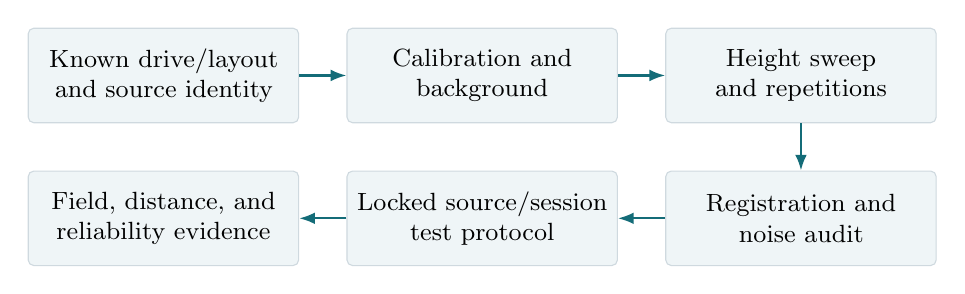
\begin{tikzpicture}[node distance=6mm]
\node[block] (src) {Known drive/layout\\and source identity};
\node[block,right=of src] (cal) {Calibration and\\background};
\node[block,right=of cal] (sweep) {Height sweep\\and repetitions};
\node[block,below=of sweep] (reg) {Registration and\\noise audit};
\node[block,left=of reg] (test) {Locked source/session\\test protocol};
\node[block,left=of test] (claim) {Field, distance, and\\reliability evidence};
\draw[arrow] (src)--(cal);\draw[arrow] (cal)--(sweep);\draw[arrow] (sweep)--(reg);
\draw[arrow] (reg)--(test);\draw[arrow] (test)--(claim);
\end{tikzpicture}
\caption{New acquisitions complement the archive. Every arrow represents a recorded processing step, so measurement improvements and network improvements can be separated.}
\end{figure}

\section{A manageable 4--6 month work plan}
\label{sec:schedule}
\begin{longtable}{P{23mm}P{65mm}P{63mm}}
\toprule Period & Main work & Exit evidence\\\midrule\endhead
Weeks 1--2 & COMSOL audit; source splits; E00--E03; request archive metadata & Trusted physics, wrong-height curves, ambiguity examples\\
Weeks 3--4 & E01/A0--A2; prior comparison; pilot learning curves & Strong known-height controls and quantitative failure diagnosis\\
Weeks 5--6 & A3 and A4; E04--E05; matched compute controls & Demonstrated benefit or rejection of joint refinement\\
Weeks 7--9 & One candidate mechanism (A5 or A6); independent literature check & A falsifiable contribution with matched ablation\\
Weeks 10--12 & E07--E09; real-data calibration/adaptation; acquisition pilot & Transfer study and stable experimental protocol\\
Weeks 13--16 & Locked evaluation; resolution and uncertainty; new height pairs & Independent evidence, failure cases, reproducibility\\
Weeks 17--20 & Paper draft; targeted reviewer-style objections; additional controls & Complete manuscript and documented limitations\\
Weeks 21--24 & Buffer for acquisition, revisions, release, and submission & A venue-ready claim matched to actual results\\\bottomrule
\end{longtable}
Dates are a planning range, not a promise. Conduct the real-data audit and acquisition scheduling early because external storage, calibration, and instrument time can be the critical path. Every week should yield a figure, table, operator check, or written decision rather than only more code.

\subsection{Weekly operating rhythm}
\begin{enumerate}
\item Write one question and a predicted outcome on Monday.
\item Run the smallest controlled experiment capable of disproving it.
\item Inspect source-level distributions, residuals, and difficult examples.
\item On Friday write a one-page conclusion with the next decision.
\item Discuss that page with collaborators; update the experiment ledger.
\end{enumerate}
Limit active modelling changes to one at a time. When a result fails, decide whether the cause is measurement physics, optimization, source prior, or unavailable information before changing capacity. The strongest result may be a reliable failure detector or a well-supported resolution limit rather than a larger neural network.

\section{From a prototype to a publishable contribution}
\label{sec:publication}
\subsection{Write the evidence chain before the paper title}
\begin{tabularx}{\linewidth}{P{35mm}YY}
\toprule Proposed claim & Evidence required & Main counterexample to test\\\midrule
Joint inference helps & A3 versus A4 with matched data/prior/compute & A larger or error-robust two-stage baseline wins\\
Handles ambiguity & Calibrated height sets; selective error & High confidence on lookalike unseen sources\\
Generalizes physically & Source/family/FOV/pitch holdouts & Hidden layout or amplitude shortcuts\\
Improves real QDM & Independent sessions/height pairs & Gains explained solely by registration\\
Recovers finer detail & Defined feature task with false positives & Plausible unsupported structure\\\bottomrule
\end{tabularx}

\subsection{Novelty audit}
For each proposed mechanism search both QDM/NV work and the broader inverse-imaging literature. Joint source--height fitting, unrolling, conditioning, Bayesian priors, and diffusion already have precedent. Write a comparison table of estimated variables, observation assumptions, prior, uncertainty, calibration, and evaluation regimes. The most important question is ``what can our method do reliably that these methods cannot under comparable information?''

Potential contributions are magnetic refinement informed by uncertainty, joint source and height inference with calibrated rejection, or an explicit treatment of unknown sources outside the FOV. These are research hypotheses. Validate novelty before writing ``first'' or ``unexplored.'' A physically rigorous benchmark can be valuable, but a narrow same-sample training score is insufficient evidence for the proposed generalization claim.

\subsection{The minimum convincing paper package}
\begin{enumerate}
\item One clearly defined problem and primary output, with observational information specified.
\item One central new mechanism or analysis, motivated by a reproducible baseline failure.
\item A simulation benchmark split by source identity/family and a real validation protocol.
\item Strong classical, direct-learned, two-stage, and joint controls under comparable information.
\item Ablations, calibration sensitivity, geometry/noise challenge sets, source-level statistics, and honest failure cases.
\item Available code/configurations/splits, or a documented substitute release if raw experimental data cannot be shared.
\end{enumerate}

Suggested paper figures: (1) ambiguity and task; (2) observation model and architecture; (3) wrong-height sensitivity; (4) baseline and joint comparisons; (5) unseen geometry/FOV/pitch; (6) uncertainty and selective risk; (7) experimental closer-plane predictions and profiles. Use only the figures supporting the actual central claim. Each caption should specify data provenance, split, physical units, and what information the method received.

\subsection{Venue strategy and dated deadline snapshot}
The following are planning judgments, not acceptance requirements or guarantees. Deadlines were checked against the linked official pages on 8 October 2026 and must be rechecked before submission.
\begin{longtable}{P{27mm}P{54mm}P{70mm}}
\toprule Venue & Deadline/status & Best emphasis for this project\\\midrule\endhead
CVPR 2027 & Registration 10 Nov 2026; paper 16 Nov 2026, AoE~\cite{cvpr} & Broadly useful blind-inference mechanism with strong physical and experimental evidence; this imminent cycle is a stretch for a new 4--6 month study.\\
ICCV 2027 & Paper deadline not confirmed on official page~\cite{iccv} & Mature method, ambiguity analysis, comprehensive transfer and real-data validation.\\
ICCP 2027 & Paper deadline not confirmed on official website~\cite{iccp} & Physics, observation modelling, self-calibration, and a new computational imaging capability.\\
ICIP 2027 & 31 Mar 2027 in IEEE SPS listing; cutoff time unconfirmed~\cite{icip} & Focused reconstruction mechanism with strong image/field evaluation and efficiency.\\
ICASSP 2027 & Regular deadline 23 Sep 2026 has passed~\cite{icassp} & A future cycle: inference/optimization method, robustness, and justified mathematical analysis.\\
EUSIPCO 2027 & 6 Feb 2027~\cite{eusipco} & Compact technical contribution; calibration or dictionary-mismatch inference.\\
Quantum 2.0 2027 & 9 Feb 2027~\cite{quantum} & Experimental quantum-sensing improvement with quantified physical benefit.\\\bottomrule
\end{longtable}
CVPR's review period overlaps the EUSIPCO deadline; do not plan simultaneous submission of substantially the same paper where prohibited. Workshop paper calls are distinct from workshop-proposal deadlines. An experimental sensing talk and an archival algorithm paper also have different publication requirements; check the actual call and prior-publication policy before planning both.

\subsection{When to stop adding experiments}
Stop architectural expansion when the central claim has reproducible support, strong alternatives have been evaluated, and the main limitations are characterized. Complete documentation, visual reporting, and the manuscript. Add a new experiment only if it resolves an objection material to the claim. A paper is improved by a coherent evidence chain, not the number of model acronyms.

\deliver{At the end of month 3, write a two-page provisional paper argument: problem, prior work, proposed mechanism, strongest figure, hardest failure, and missing decisive evidence. Use it to choose the final venue and remaining acquisitions.}

\appendix
\section{Implementation map for the current repository}
\label{sec:implementation}
\subsection{What can be reused}
\begin{tabularx}{\linewidth}{P{51mm}Y}
\toprule Existing file/area & Reuse and required distinction\\\midrule
\texttt{scripts/propagator.py} & Physical frequency convention and analytic transfer; extend observation modelling in a separate experiment.\\
\texttt{scripts/iterative.py} & Comparable ISTA/FISTA, objective/stationarity diagnostics, epsilon stopping, honest stop reasons.\\
\texttt{scripts/torch\_inverse.py} & FFT mechanics and adjoint checks; current transfer is fixed and single-channel, so a dynamic height operator needs a new implementation.\\
\texttt{scripts/lista.py} & Initialization-equivalent learned corrections, tied weights, checkpoint patterns, trained-depth semantics.\\
\texttt{scripts/compare\_lista.py} & Training/timing/provenance patterns; replace same-sample kernel fitting, truth-derived scaling, and training-only selection in the new benchmark.\\
\texttt{tests/} & Existing numerical checks; extend only where new operator contracts, derivatives, projections, and sampling change.\\
Crop and lambda reports & Useful diagnostics and historical experiments; direct periodic crops are not a replacement for the new finite-window benchmark.\\\bottomrule
\end{tabularx}
Retain archived outputs. The proposed work is a new protocol and should not be compared as if old fixed-iteration, empirical-kernel, same-sample runs used the same observation information. The existing COMSOL cache naming does not encode geometry identity; the expanded database requires a different manifest/key scheme.

Suggested new modules: \texttt{dataset\_manifest.py}, \texttt{observation\_model.py}, \texttt{joint\_models.py}, \texttt{train\_joint.py}, \texttt{evaluate\_joint.py}, and \texttt{report\_joint.py}. These names describe a possible future organization; this document has not created or validated that training pipeline.

\subsection{A differentiable propagation fragment}
This example handles a symmetric padded field operator only. Projection, pixel integration, unequal latent/observation support, masks, and whitening must be composed separately with their correct adjoints. It demonstrates that the transfer is computed from a tensor height without converting it to NumPy or detaching it.
\par\noindent\begin{minipage}{\linewidth}
\begin{lstlisting}[language=Python]
import torch
import torch.nn.functional as F

def propagate(x, h, dx_um, z_ref_um=0.5, pad=32):
    # x: [batch, channels, H, W], signed fields
    # h: [batch], in um, kept in the autograd graph
    # dx_um: common physical pitch for this batch
    H0, W0 = x.shape[-2:]
    xp = F.pad(x, (pad, pad, pad, pad)) if pad else x
    ny, nx = xp.shape[-2:]
    fy = torch.fft.fftfreq(ny, d=dx_um,
                          device=x.device, dtype=x.dtype)
    fx = torch.fft.fftfreq(nx, d=dx_um,
                          device=x.device, dtype=x.dtype)
    freq = torch.sqrt(fy[:, None]**2 + fx[None, :]**2)
    gap = (h - z_ref_um).reshape(-1, 1, 1, 1)
    transfer = torch.exp(-2 * torch.pi * gap * freq)
    out = torch.fft.ifft2(torch.fft.fft2(xp) * transfer).real
    return out[..., pad:pad + H0, pad:pad + W0]

# Validate positive gaps and pitch in the caller.
# Cache frequency grids by shape/pitch/device/dtype, not H(h).
# Different dx and dy require separate frequency spacings.
\end{lstlisting}
\end{minipage}\par
For the same real radial transfer and symmetric support, the adjoint has the same pad/convolve/crop form. That statement does not extend automatically to arbitrary $\C$, $\Samp$, or $\mathcal Q$; their adjoints must insert residuals, transpose averaging, and transpose projection in reverse order. Check the implemented operator rather than assuming a transpose from its diagram.

\subsection{A split-aware training skeleton}
\begin{lstlisting}[language=Python]
for batch in train_loader:
    y, truth, h_true, metadata = batch
    # metadata contains only information allowed at inference
    x_hat, h_hat = model(y, metadata)
    y_hat = observation_model(x_hat, h_hat, metadata)
    loss = field_loss(x_hat, truth)
    loss += weight_h * height_loss(h_hat, h_true)
    loss += weight_obs * observation_loss(y_hat, y, metadata)
    optimizer.zero_grad()
    loss.backward()
    optimizer.step()

# Select checkpoints using held-out validation sources.
# Fit uncertainty calibration on a separate calibration split.
# Evaluate the locked source/session test split after selection.
\end{lstlisting}
The fragment is conceptual. It does not specify a novel architecture, justify the noise likelihood, or guarantee convergence. Simulation height labels are training supervision; never substitute true test height for a predicted estimate in the unknown-height result.

\clearpage
\section{Practical records and templates}
\subsection{Scene manifest example}
\par\noindent\begin{minipage}{\linewidth}
\begin{lstlisting}
geometry_id: cad_hash_or_stable_layout_id
scene_id: geometry_drive_mesh_id
source_family: spiral_or_other_declared_family
source_plane_definition: conductor_top_surface
reference_height_um: 0.5
observation_height_um: 3.0
height_label_kind: exact_simulation_coordinate
height_uncertainty_um: 0.0
dx_um: 0.1
dy_um: 0.1
field_quantity: B
field_unit: T
components: [Bx, By, Bz]
current_A: measured_or_prescribed_value
grid_shape: [ny, nx]
simulation_mesh_id: mesh_hash
split_group: geometry_id_or_template_family
parent_scene: full_physical_scene_id
observation_transform: sensing_then_crop_version
acquisition_session: null_for_simulation
\end{lstlisting}
\end{minipage}\par
This example uses existing project units and a sample height pair. It is not a claim that every external database entry has those values. An experimental manifest should add NV axis, stage increments, absolute-height calibration method, raw-data references, lock-in/ODMR settings, drive logs, and measurement covariance identifiers.

\subsection{Experiment card}
\begin{tcolorbox}
\textbf{ID and question:}\quad E\_\_\_ / What would this experiment establish?\par
\textbf{Hypothesis and falsifier:}\quad What outcome would reject the explanation?\par
\textbf{Inputs at inference:}\quad Height? CAD? dictionary? projection? pitch?\par
\textbf{Data and split:}\quad Source groups, acquisition sessions, manifest hashes.\par
\textbf{Method/control:}\quad One change; matched prior/data/compute.\par
\textbf{Primary endpoint:}\quad Field, height, resolution, or reliability criterion.\par
\textbf{Secondary diagnostics:}\quad Residual maps, profiles, spectra, timing.\par
\textbf{Result and uncertainty:}\quad Source-level effect size and confidence interval.\par
\textbf{Decision:}\quad Keep, reject, investigate physics, or acquire missing data.
\end{tcolorbox}

\subsection{First 10 working days}
\begin{enumerate}
\item Days 1--2: inventory the existing COMSOL database; define source identities, height origin, units, and available targets. Request the experimental archive and logs.
\item Days 3--4: freeze a pilot split; validate analytical propagation, adjoints, and height derivatives against small cases and several COMSOL pairs.
\item Days 5--6: produce known-height classical reconstructions and the wrong-height sweep. Examine boundary and spectral errors.
\item Days 7--8: form source--height lookalike pairs; vary source size/current independently. Write the ambiguity diagnosis.
\item Days 9--10: train a small known-height learned baseline or height predictor, depending on the diagnosis; draft the one-page next-experiment argument.
\end{enumerate}
The timetable assumes the COMSOL files can be read and paired. If the audit reveals inconsistent coordinates or missing targets, those corrections become the first milestone. Do not start a month-long training campaign before the input contract is trusted.

\subsection{Failure triage}
\begin{tabularx}{\linewidth}{P{42mm}Y}
\toprule Symptom & First investigation\\\midrule
Height runs to a bound & Non-identifiability, amplitude scaling, prior bias, sign of height derivative\\
Residual improves; truth worsens & Regularization, unstable frequencies, wrong model, invalid height information\\
Crop seams or edge rings & Periodic assumption, source outside FOV, padding/support mismatch\\
Wrong amplitudes/signs & Units, normalization, NV projection, current sign, final activation\\
Good simulations; poor real maps & Registration, covariance, optical/NV averaging, raw readout artifacts\\
Uncertainty always tiny & Calibration leakage, narrow training family, unjustified likelihood, branch collapse\\
Uncertainty always broad & Poor scores, insufficient information, candidate spacing, untrained prior\\
Joint model loses to two-stage & Weak control tuning, noisy height updates, redundant mechanism, excessive complexity\\\bottomrule
\end{tabularx}

\subsection{A final claim audit}
Before submission, ask whether the novelty is an algorithm, an uncertainty method, an observation model, or an experimental capability. State what was given at inference and what was estimated. Describe which fine features were validated independently, which depend on priors, and whether the height reference is absolute or relative. Make ``unseen geometry'' mean excluded physical identities, not new crops of the same coil. Make ``super-resolution'' mean a defined physical detail-recovery result, not a larger tensor.

\section{Focused reading and questions for collaborators}
\subsection{Read with an implementation target}
\begin{enumerate}
\item \textbf{LISTA and ALISTA:} derive the layer from a proximal iteration and reproduce initialization equivalence~\cite{lista,alista}.
\item \textbf{U-Net and FiLM:} build a multiscale signed-field baseline, then test a single metadata-conditioning change~\cite{unet,film}.
\item \textbf{MoDL/VarNet:} implement exact data consistency for this observation model instead of copying the MRI encoding~\cite{modl,varnet}.
\item \textbf{QDM current reconstruction:} identify the actual observation components, priors, and standoff/noise comparisons~\cite{midha,reed,broadway}.
\item \textbf{Bathla dictionary work:} reproduce the available-data task and distinguish coefficient sparsity from field-pixel sparsity~\cite{bathla}.
\item \textbf{Joint calibration and Bayesian source inference:} map which assumptions stabilize the inverse~\cite{setescak,clement,blinddps}.
\item \textbf{Calibration:} implement coverage and selective-risk evaluation before adding a more complex posterior network~\cite{guo,conformal}.
\end{enumerate}

\subsection{Questions to resolve when the hard disk arrives}
\begin{itemize}
\item Which maps are raw measurements, fitted fields, averaged references, or dictionary reconstructions?
\item Are all original basis maps and activation/drive labels available, and are actual currents recorded?
\item Are there repeated acquisitions, current-off data, raw fit residuals, and timestamps?
\item Were heights independently calibrated, or estimated by a model? Which coordinate is the origin?
\item Which coils and layer depths are known, and which CAD variants have corresponding COMSOL models?
\item Do the archive's measurements include a usable closer-plane reference, or should we acquire one?
\item Which arrays/sessions can be withheld for adaptation, calibration, and final testing?
\end{itemize}
These questions are operational metadata requirements. They do not require changing the agreed primary target or delaying the simulation pilot.

\begingroup\small
\begin{thebibliography}{99}
\setlength{\itemsep}{3pt}
\setlength{\parskip}{0pt}
\bibitem{lista} K. Gregor and Y. LeCun. \emph{Learning Fast Approximations of Sparse Coding}. ICML, 2010. \url{https://icml.cc/Conferences/2010/papers/449.pdf}.
\bibitem{alista} J. Liu, X. Chen, Z. Wang, and W. Yin. \emph{ALISTA: Analytic Weights Are As Good As Learned Weights in LISTA}. ICLR, 2019. \url{https://openreview.net/forum?id=B1lnzn0ctQ}.
\bibitem{unet} O. Ronneberger, P. Fischer, and T. Brox. \emph{U-Net: Convolutional Networks for Biomedical Image Segmentation}. 2015. \url{https://arxiv.org/abs/1505.04597}.
\bibitem{film} E. Perez et al. \emph{FiLM: Visual Reasoning with a General Conditioning Layer}. AAAI, 2018. \url{https://arxiv.org/abs/1709.07871}.
\bibitem{modl} H. K. Aggarwal, M. P. Mani, and M. Jacob. \emph{MoDL: Model Based Deep Learning Architecture for Inverse Problems}. IEEE Transactions on Medical Imaging, 2018. \url{https://arxiv.org/abs/1712.02862}.
\bibitem{varnet} A. Sriram et al. \emph{End-to-End Variational Networks for Accelerated MRI Reconstruction}. 2020. \url{https://arxiv.org/abs/2004.06688}.
\bibitem{nafnet} L. Chen et al. \emph{Simple Baselines for Image Restoration}. ECCV, 2022. \url{https://arxiv.org/abs/2204.04676}.
\bibitem{dip} D. Ulyanov, A. Vedaldi, and V. Lempitsky. \emph{Deep Image Prior}. CVPR, 2018. \url{https://arxiv.org/abs/1711.10925}.
\bibitem{pnp} S. V. Venkatakrishnan, C. A. Bouman, and B. Wohlberg. \emph{Plug-and-Play Priors for Model Based Reconstruction}. GlobalSIP, 2013. \url{https://brendt.wohlberg.net/publications/venkatakrishnan-2013-plugandplay.html}.
\bibitem{fno} Z. Li et al. \emph{Fourier Neural Operator for Parametric Partial Differential Equations}. ICLR, 2021. \url{https://arxiv.org/abs/2010.08895}.
\bibitem{blinddps} H. Chung, J. Kim, S. Kim, and J. C. Ye. \emph{Parallel Diffusion Models of Operator and Image for Blind Inverse Problems}. CVPR, 2023. \url{https://arxiv.org/abs/2211.10656}.
\bibitem{guo} C. Guo, G. Pleiss, Y. Sun, and K. Q. Weinberger. \emph{On Calibration of Modern Neural Networks}. ICML, 2017. \url{https://arxiv.org/abs/1706.04599}.
\bibitem{conformal} A. N. Angelopoulos and S. Bates. \emph{A Gentle Introduction to Conformal Prediction and Distribution-Free Uncertainty Quantification}. 2021. \url{https://arxiv.org/abs/2107.07511}.
\bibitem{broadway} D. A. Broadway et al. \emph{Improved Current Density and Magnetization Reconstruction Through Vector Magnetic Field Measurements}. Physical Review Applied 14, 024076, 2020. \url{https://arxiv.org/abs/2005.06788}.
\bibitem{midha} S. Midha et al. \emph{Optimized Current Density Reconstruction from Widefield Quantum Diamond Magnetic Field Maps}. Physical Review Applied 22, 014015, 2024. \url{https://arxiv.org/abs/2402.17781}.
\bibitem{reed} N. R. Reed et al. \emph{Machine Learning for Improved Current-Density Reconstruction from Two-Dimensional Vector Magnetic Images}. Physical Review Applied 23, 034035, 2025. \url{https://arxiv.org/abs/2407.14553}.
\bibitem{bathla} A. Bathla, M. Parashar, M. Markham, A. Rajwade, and K. Saha. \emph{Dictionary-Based Reconstruction of Spatio-Temporal 3D Magnetic Field Images from Quantum Diamond Microscope}. Preprint, 2025; published in Optica 13, 686--697, 2026. The archive protocol here refers to the linked preprint description. \url{https://arxiv.org/html/2506.05491v1}.
\bibitem{setescak} A. Setescak et al. \emph{A Fourier-Space Approach to Physics-Informed Magnetization Reconstruction from Nitrogen-Vacancy Measurements}. arXiv:2602.17180v3, 2026. \url{https://arxiv.org/abs/2602.17180}.
\bibitem{clement} C. B. Clement, J. P. Sethna, and K. C. Nowack. \emph{Reconstruction of Current Densities from Magnetic Images by Bayesian Inference}. 2021 version. \url{https://arxiv.org/abs/1910.12929}.
\bibitem{qdsim} S. Pandey et al. \emph{QDsiM: A Noise-Aware Simulation Toolkit for Quantum Diamond Microscope}. Preprint, 2026. \url{https://arxiv.org/abs/2601.11649}.
\bibitem{cvpr} CVPR 2027 official call for papers. Checked 8 October 2026. \url{https://cvpr.thecvf.com/Conferences/2027/CallForPapers}.
\bibitem{iccv} ICCV 2027 official dates page. Checked 8 October 2026. \url{https://iccv.thecvf.com/Conferences/2027/Dates}.
\bibitem{iccp} ICCP 2027 official website. Checked 8 October 2026. \url{https://iccp2027.iccp-conference.org/}.
\bibitem{icip} IEEE Signal Processing Society ICIP listing. Checked 8 October 2026. \url{https://signalprocessingsociety.org/event-names/icip}.
\bibitem{icassp} ICASSP 2027 official important dates. Checked 8 October 2026. \url{https://2027.ieeeicassp.org/important-dates/}.
\bibitem{eusipco} EUSIPCO 2027 official website. Checked 8 October 2026. \url{https://eusipco2027.de/}.
\bibitem{quantum} Optica Quantum 2.0 official call. Checked 8 October 2026. \url{https://www.optica.org/events/topical_meetings/quantum/}.
\end{thebibliography}
\endgroup

\end{document}
